\begin{itemize}
    \item Beschreibt die Grundüberlegungen der realisierten Lösung (Konstruktion/Entwurf) und die Realisierung als Simulation, als Prototyp oder als Software-Komponente etc.
    \item Hier beschreiben Sie Ihre gemachte Arbeit. Dazu braucht es eine Beschreibung des Vorgehens, aller Arbeitsschritte usw.
    \item (Definiert Messgrössen, beschreibt Mess- oder Versuchsaufbau, beschreibt und dokumentiert Durchführung der Messungen/Versuche)
    \item Bildmaterial erleichtert das Verständnis.
    \item (Experimente)
    \item Immer mit Aufbau und Vorgehen; Bildmaterial erleichtert das Verständnis.
    \item (Lösungsweg)
    \item Inkl. theoretische Herleitung der Lösung
    \item (Modell)
    \item (Eingesetzte Software)
    \item Die Funktionen von verwendeten Computerprogrammen zu Simulationszwecken, Berechnungen etc. sollen beschrieben werden. Dies soll aber in Worten, Formeln und geeigneten Darstellungen (z.B. Fluss- diagrammen) geschehen. Allfälliger Programmcode ist in einem Anhang zu dokumentieren.
    \item (Tests und Validierung)
\end{itemize}

\textbf{Marco's Proposal}
\begin{itemize}
    \item Anfangs High Level Overview Mischung, Kapitel ersichtlich was kommt Flussdiagram (um dieses haben wir dann die Prozessmethoden)
    \item Vorgehensmethode => Kanban und Scrum, maybe V-Model?
    \item Setup technisch, lokale Linux VM, ROS Installation, VS Code als IDE, GitHub Repos, GitHub Actions CI/CD (maybe?), Deployment Architektur
    \item Overview Architektur ROS und Code, Grundüberlegung => Path Planning Package in ROS, Prototyp Architektur zeigen, Explo und Opt Algos, erhaltet Input und sendet Input
    \item Messages (interfaces und fszhaw msgs) (System aussen)
    \item Path Planner Node
    \item Exploration Algorithm
    \item Optimization Service Node
    \item Optimization Algorithm
    \item Verifikation und Validierungen (Code Reviews, Fehlerfälle: Cones gehen verloren, Cones andere Seite entdeckt, allg Fehlerannahmen)
    \item Testing mit Maps, Cone Publisher und Planned Trajectory Subscriber (mocks), utils wie track plotter, trackconfig
    \item Setup eher im Projektanhang: Weekly meetings, Review every other week, Mitarbeit mit anderen BA Teams in Driverless und gesamt Verein (Working Saturday, Hilfe im Workshop, Ausstellung Conecto ZHAW)
    \item In Resultate Kapitel, Vergleich erste Algorithmen und Versuche: erste Überlegungen und Tests, alter path planner zhaw, dann densify und interpolate, rrt max hamburg, komplexer algo à la ultimate und dann jetzige implementation, zuerst was hat eth mit mpcc, dann global racetrajectory von tumftm
\end{itemize}

This chapter describes the approaches and methods used to solve the problem of finding algorithms that calculate the optimum path on a race track. The V-Model was used to plan the overall project as shown in figure \ref{fig:High Level Project Overview}. Concepts of Scrum were used for the interdisciplinary work between the different Driverless teams and within the Path Planning team itself. Sprint planning and review meetings were held with the supervisors and the driverless teams. Further explanation of the planning process is described in the section \ref{sec:Planning Methods}. After the planning section, the development environment is described in section \ref{sec:Development Environment}. Then an introduction to the architecture design of the Path Planning component is explained in section \ref{sec:Path Planning Component Architecture}. The algorithms are explained in section \ref{sec:Exploration Algorithm} for the exploration and section \ref{sec:Optimization Algorithm} for the optimization algorithm. Lastly, the integration and verification process is described in section \ref{sec:Integration and Verification}.

\begin{figure}[H]
    \centering
    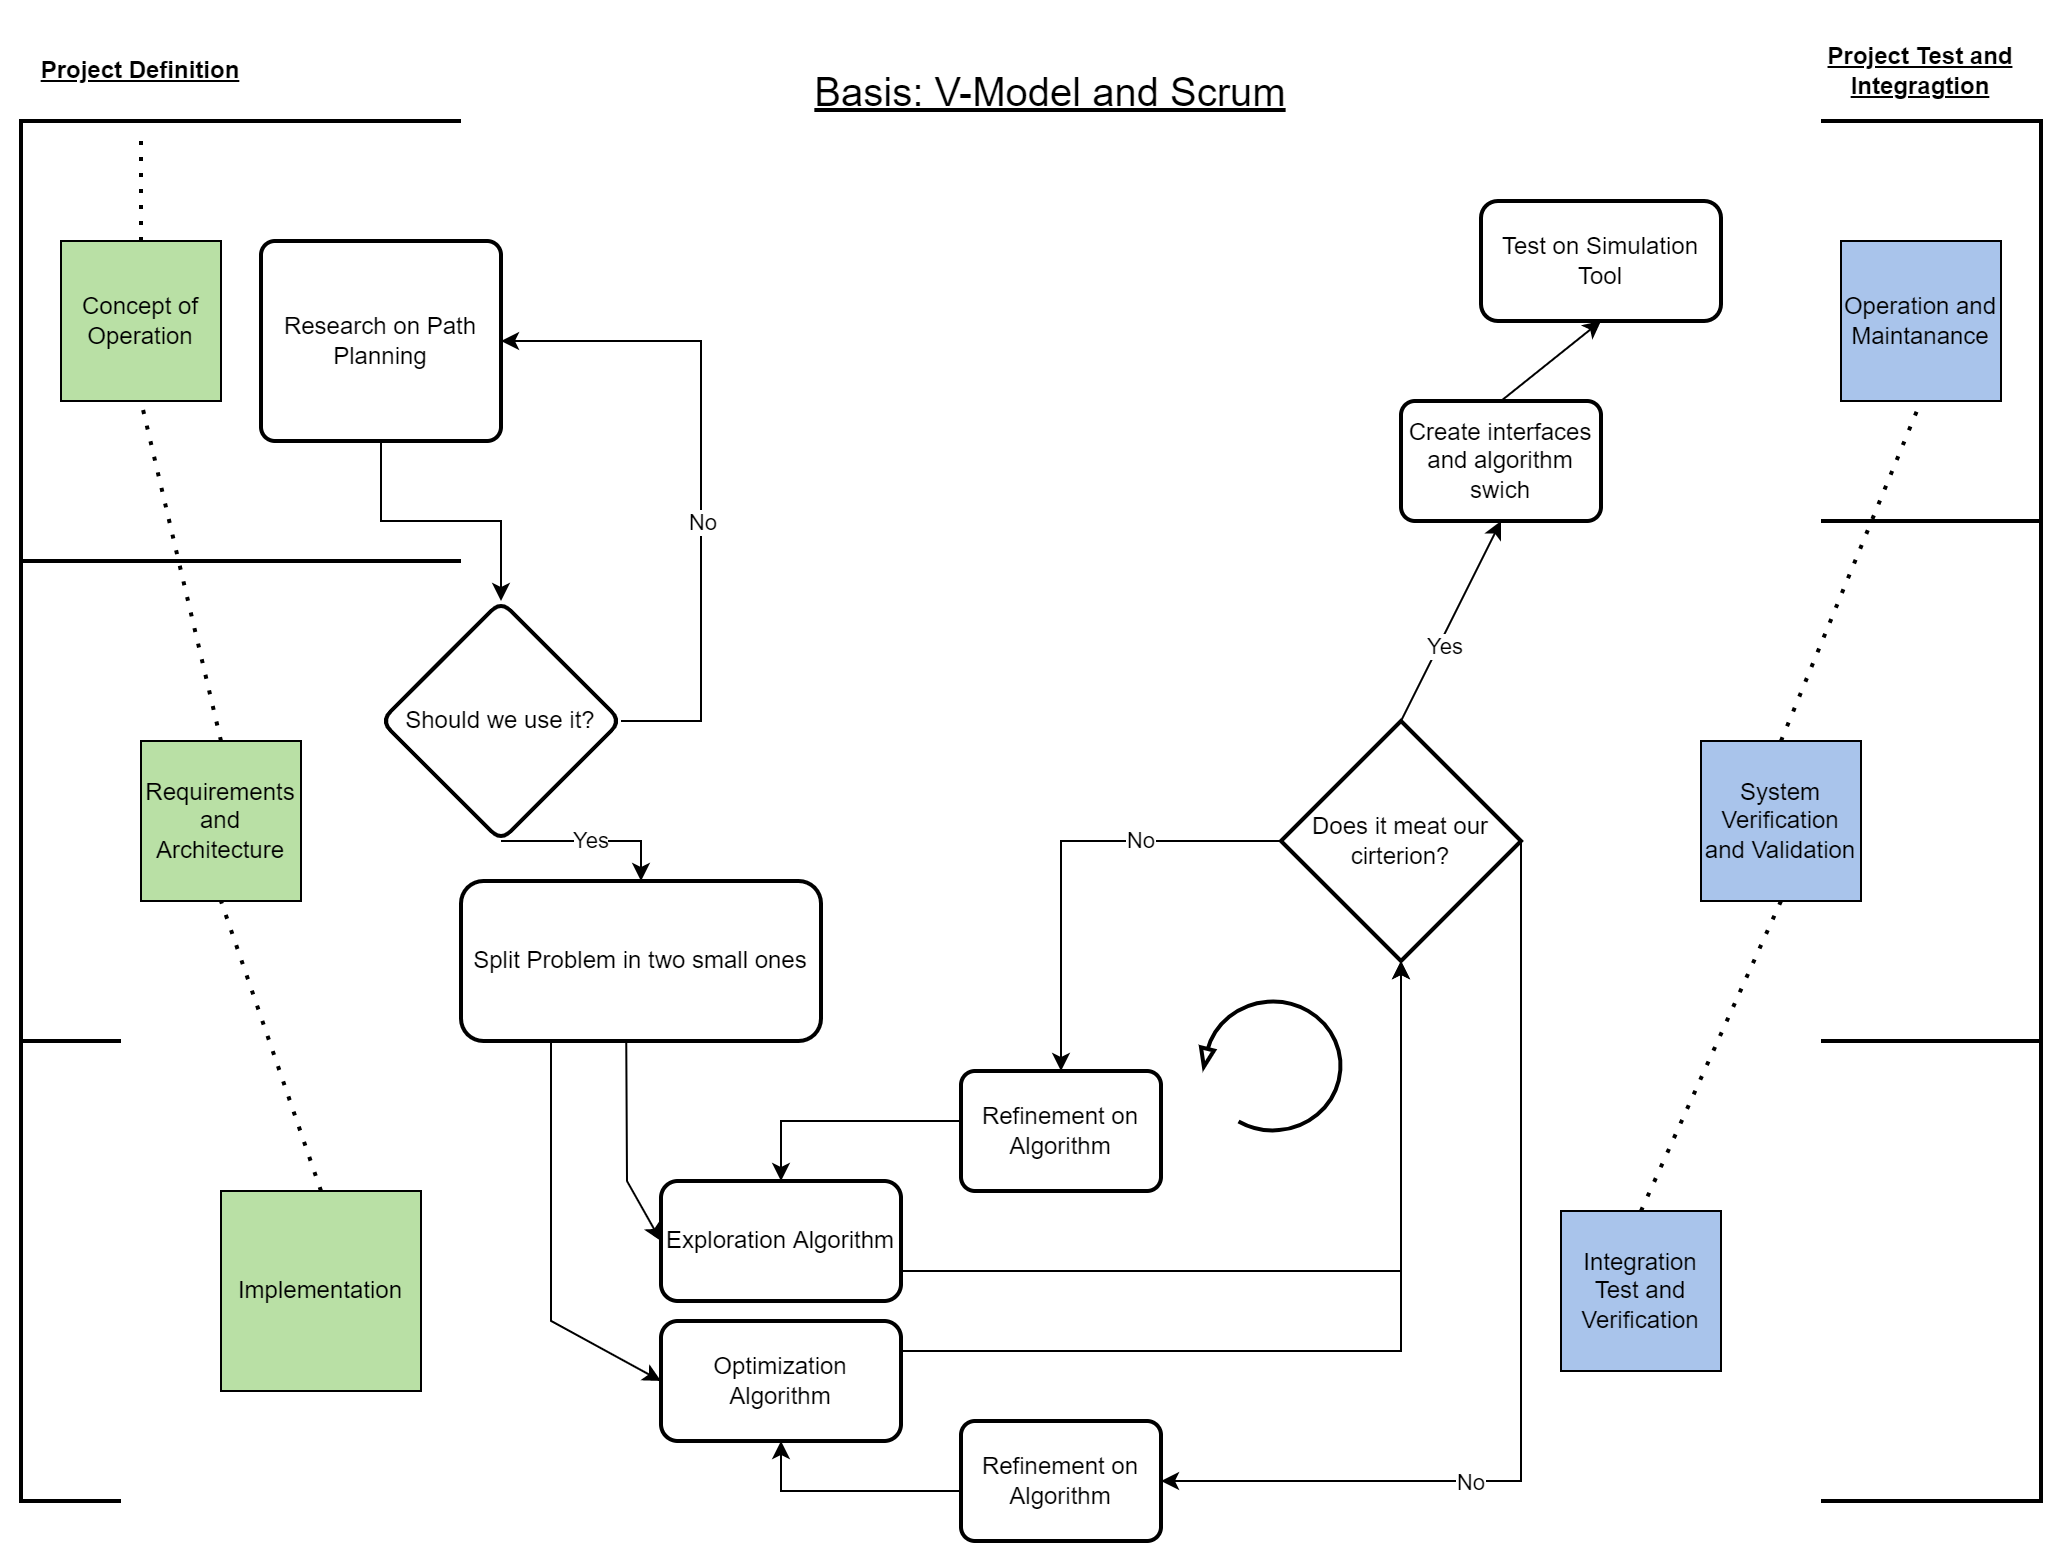
\includegraphics[width=\columnwidth]{High_Level_Project_Overview.png}
    \caption{The high-level project overview illustrates which approaches and methods have been used to realize the project.}
    \label{fig:High Level Project Overview}
\end{figure}

\section{Planning Methods} \label{sec:Planning Methods}
Often, planning methods are used for accomplishing complex tasks within a team. In modern Software Engineering, Scrum is ubiquitous as an agile planning method. As for the overall project plan, the V-Model was used.

\subsection{V-Model} \label{sec:Planning Method: V-Model}
The V-Model consists of several stages as shown in figure \ref{fig:V-Model}.
\begin{figure}[H]
    \centering
    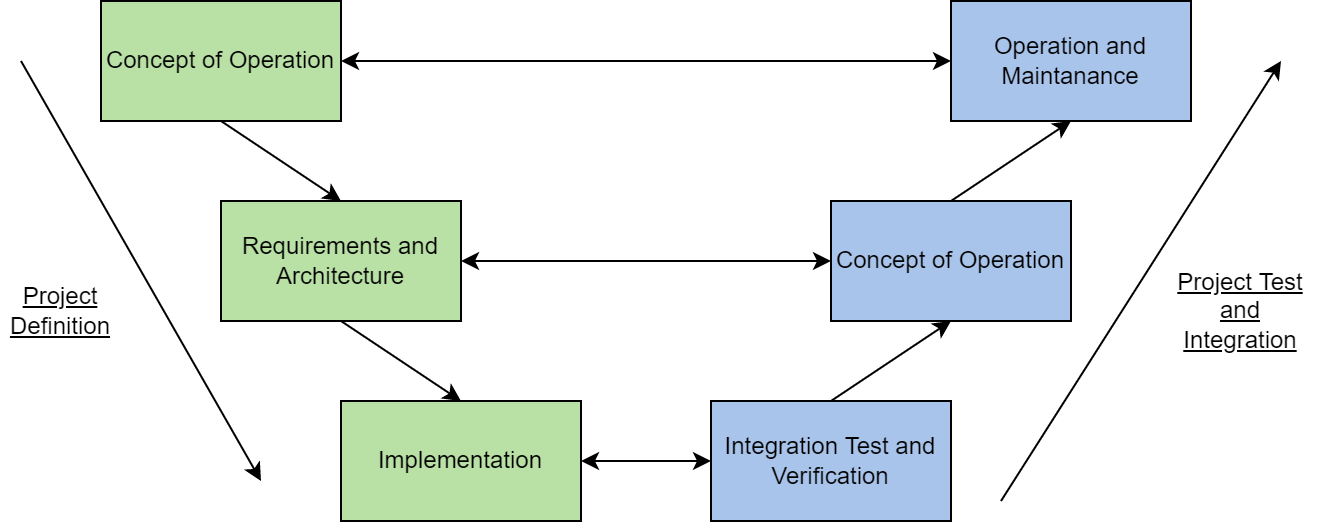
\includegraphics[width=\columnwidth]{V-Model.png}
    \caption{The V-Model helps in an IT-Project to have a focus on planning and implementation while reflecting and testing the program.}
    \label{fig:V-Model}
\end{figure}

It starts with the concept of the operation stage. Making the first plan and conducting research is done during this stage. Second, deciding on the requirements and architecture is done. These steps cover the process of building a development system that is near the production environment. In this project, the production system will be the NVIDIA Jetson, which will be inside the DV box as seen in figure \ref{fig:AS DV Box} in section \ref{sec:Zurich UAS Racing Autonomous System}.
In contrast, the development system is a \acrlong{vm}. Splitting the problem to find an optimum path into two smaller ones like the exploration and optimization algorithm helped divide the workload and have the four-eye principle on each other's code. The last part covers implementing the algorithms in the development environment and testing it. During implementation, definitions of how to test these algorithms and verify a good one from a bad one have to be done. The integration and verification are covered in chapter \ref{ch:Results}. The concept of the Operation process consists of the evaluation of the algorithms if they fit the criterion. Lastly, the operation and maintenance phase integrates the algorithms into the production system.

\subsection{Scrum} \label{sec:Planning Method: Scrum}
Scrum was used as a project management framework between the supervisors and the developers. An explanation of how Scrum works can be found in the appendix under \ref{sec:Scrum}. Weekly meetings were held with the supervisors and biweekly with the driverless team. In addition, the team itself held a meeting every week as well. Before such a meeting, the team would send an e-mail containing an update of last week's progress. User stories were directly created from the meeting notes.

A kanban board helps organize the user stories and prioritize the stories in the development process. As shown in figure \ref{fig:Kanban Board Path Planning}, there are four columns. The ``To Do'' list with the available inputs and ideas. The ``In progress'' list shows the current tasks, and the ``Review in progress'' shows completed tasks the other team member can review. Finally, the ``Done'' column shows all finished tasks. One Kanban board was created to develop the Path Planning implementation, while another Kanban board was created just for writing the thesis.
\begin{figure}[H]
    \centering
    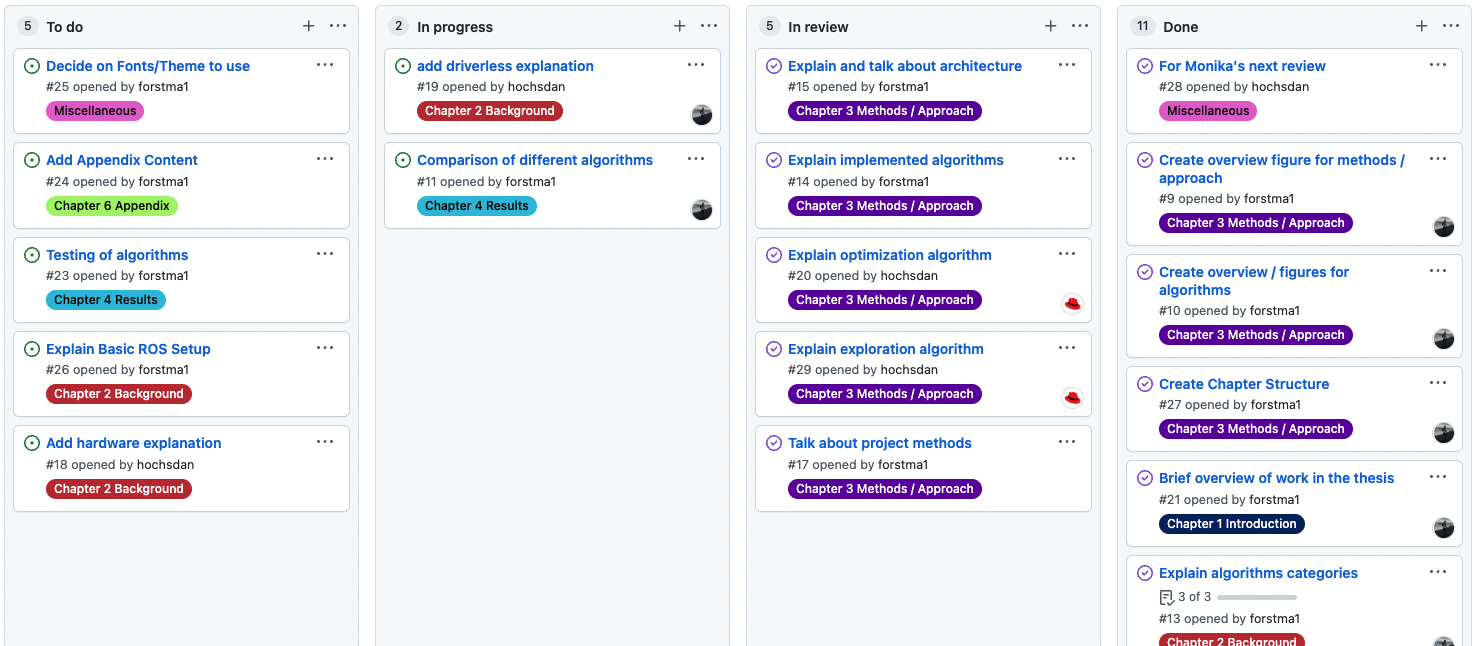
\includegraphics[width=\columnwidth]{Kanban_Board_Path_Planning.PNG}
    \caption{The Kanban Board directly integrated into GitHub used for the bachelor thesis.}
    \label{fig:Kanban Board Path Planning}
\end{figure}

\section{Development Environment} \label{sec:Development Environment}
An easy way to get started with an environment was to build a relatively similar system like the one which will be running on the NVIDIA Jetson computer, as previously seen in figure \ref{fig:AS Deployment Diagram}. As mentioned in the planning methods section \ref{sec:Planning Methods}, the Jetson will be used in the real car.
For the local development, the underlying hardware differs from user to user; this can be a desktop PC at home or a portable notebook. On top of the hardware runs the user's operating system, which can be running a standard Windows installation, macOS or even a Linux installation. Inside the host's operating system, a \acrlong{vm} is used to emulate the hardware and to encapsulate the operating system from the host operating system that is running on the actual hardware. As with the NVIDIA Jetson computer, an Ubuntu 20.04 operating system was installed. An installation guide for how to install Ubuntu 20.04 in a \acrshort{vm} can be found at Cloud Linux Tech. \cite{cloudlinuxtech_install_ubuntu_2004} The work done in this thesis has been done using the ROS 2 release 'Foxy Fitzroy', released on June 5th, 2020. This release will be supported till the end of May 2023. \cite{ros2_releases_and_target_platforms}
Figure \ref{fig:Development Environment} shows the overall environment that is used for development.
\begin{figure}[H]
    \centering
    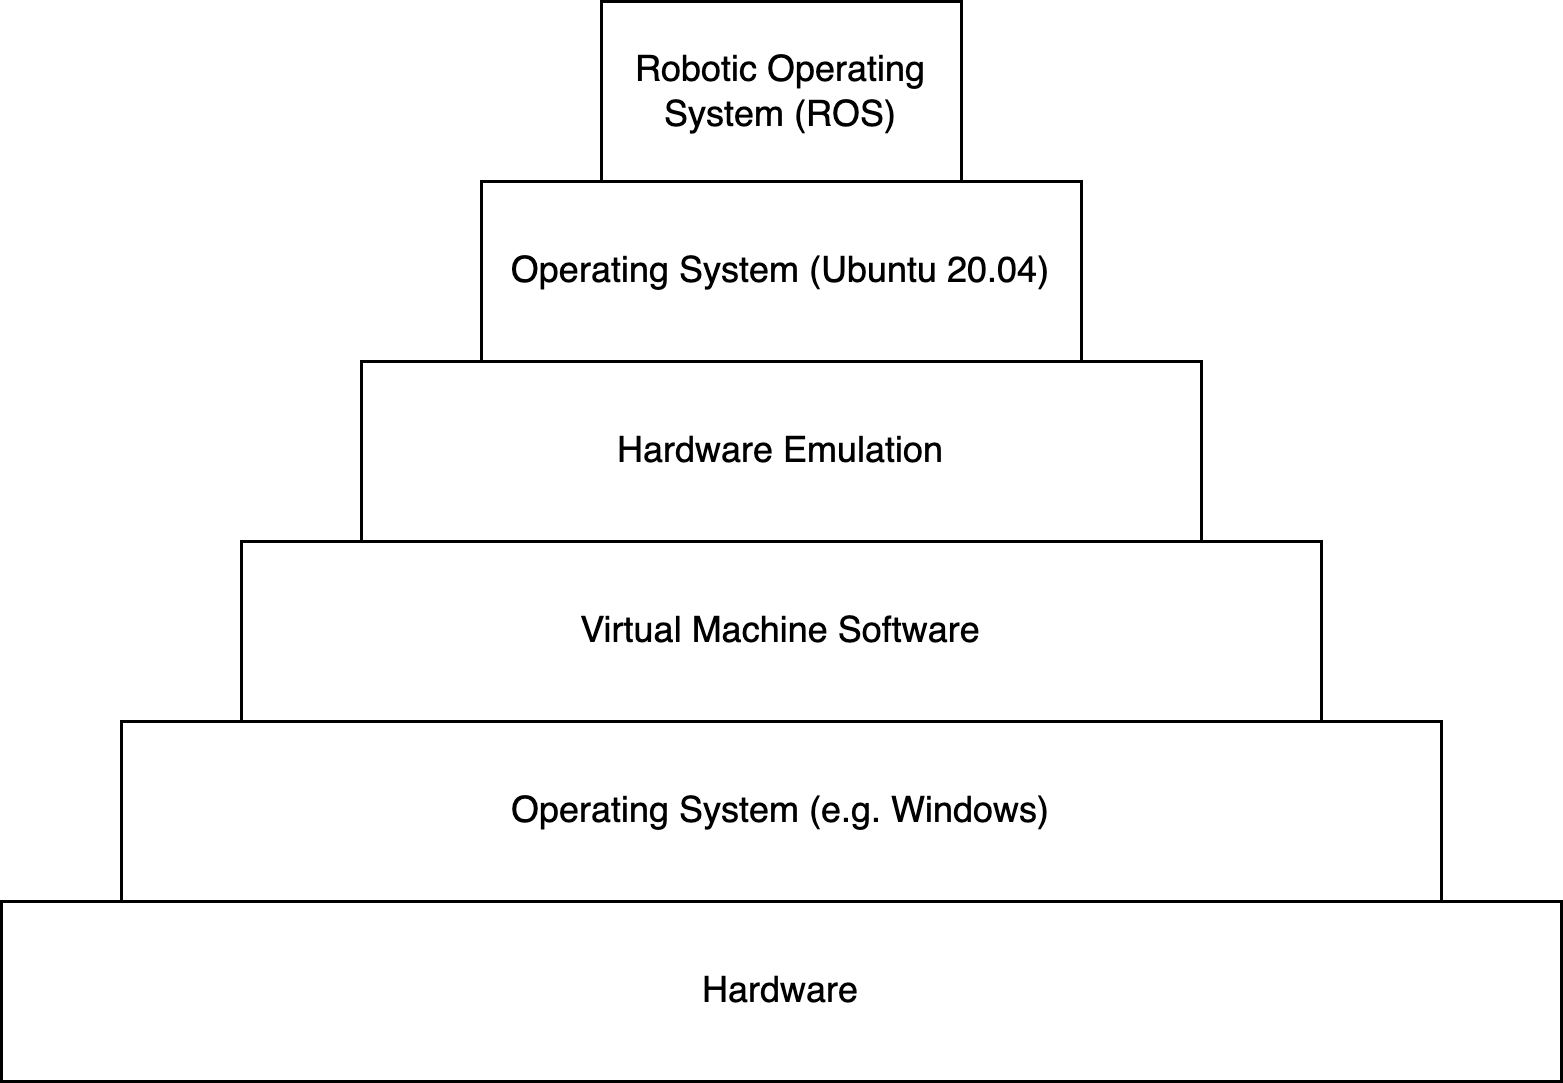
\includegraphics[width=10cm]{Development_Architecture.png}
    \caption{The development environment consists of various layers: the hardware, the host operating system, the \acrshort{vm}, the operating system on the \acrshort{vm} and the \acrshort{ros} installation.}
    \label{fig:Development Environment}
\end{figure}

\subsection{Integrated Development Environment (IDE) and Version Control} \label{sec:Integrated Development Environment (IDE) and Version Control}
An Integrated Development Environment (IDE) called Visual Studio Code was used to develop the Path Planner. The IDE provides functionalities like syntax checking on Python and C++ code. Furthermore, the IDE was used to write the thesis in Latex. An extension inside Visual Studio Code can be installed to generate PDF files via Latex. A separate Git Repository for version control was created for both the code and the thesis. The version control system helps a software engineering team follow changes in the code, and in case of any problem, it can be jumped back to an older version of the code. The Git server hosted by the \acrshort{zhaw} was used to store the repositories (\href{https://github.zhaw.ch}{github.zhaw.ch}).

\section{Path Planning Component Architecture} \label{sec:Path Planning Component Architecture}
This section will give an overview of the Path Planning component as seen in the component Autonomous System Component diagram \ref{fig:AS Component Diagram}. The Path Planner will receive its inputs by Perception (detected cones) and Localization/Odometry (current position) via the Mapping and send its output (planned path) to the Autopilot component.

The path planning component primarily consists of two \acrshort{ros} nodes: The 'Path Planner' node and the 'Optimization Service' node, as seen in figure \ref{fig:Path Planning ROS Architecture}.
\begin{figure}[H]
    \centering
    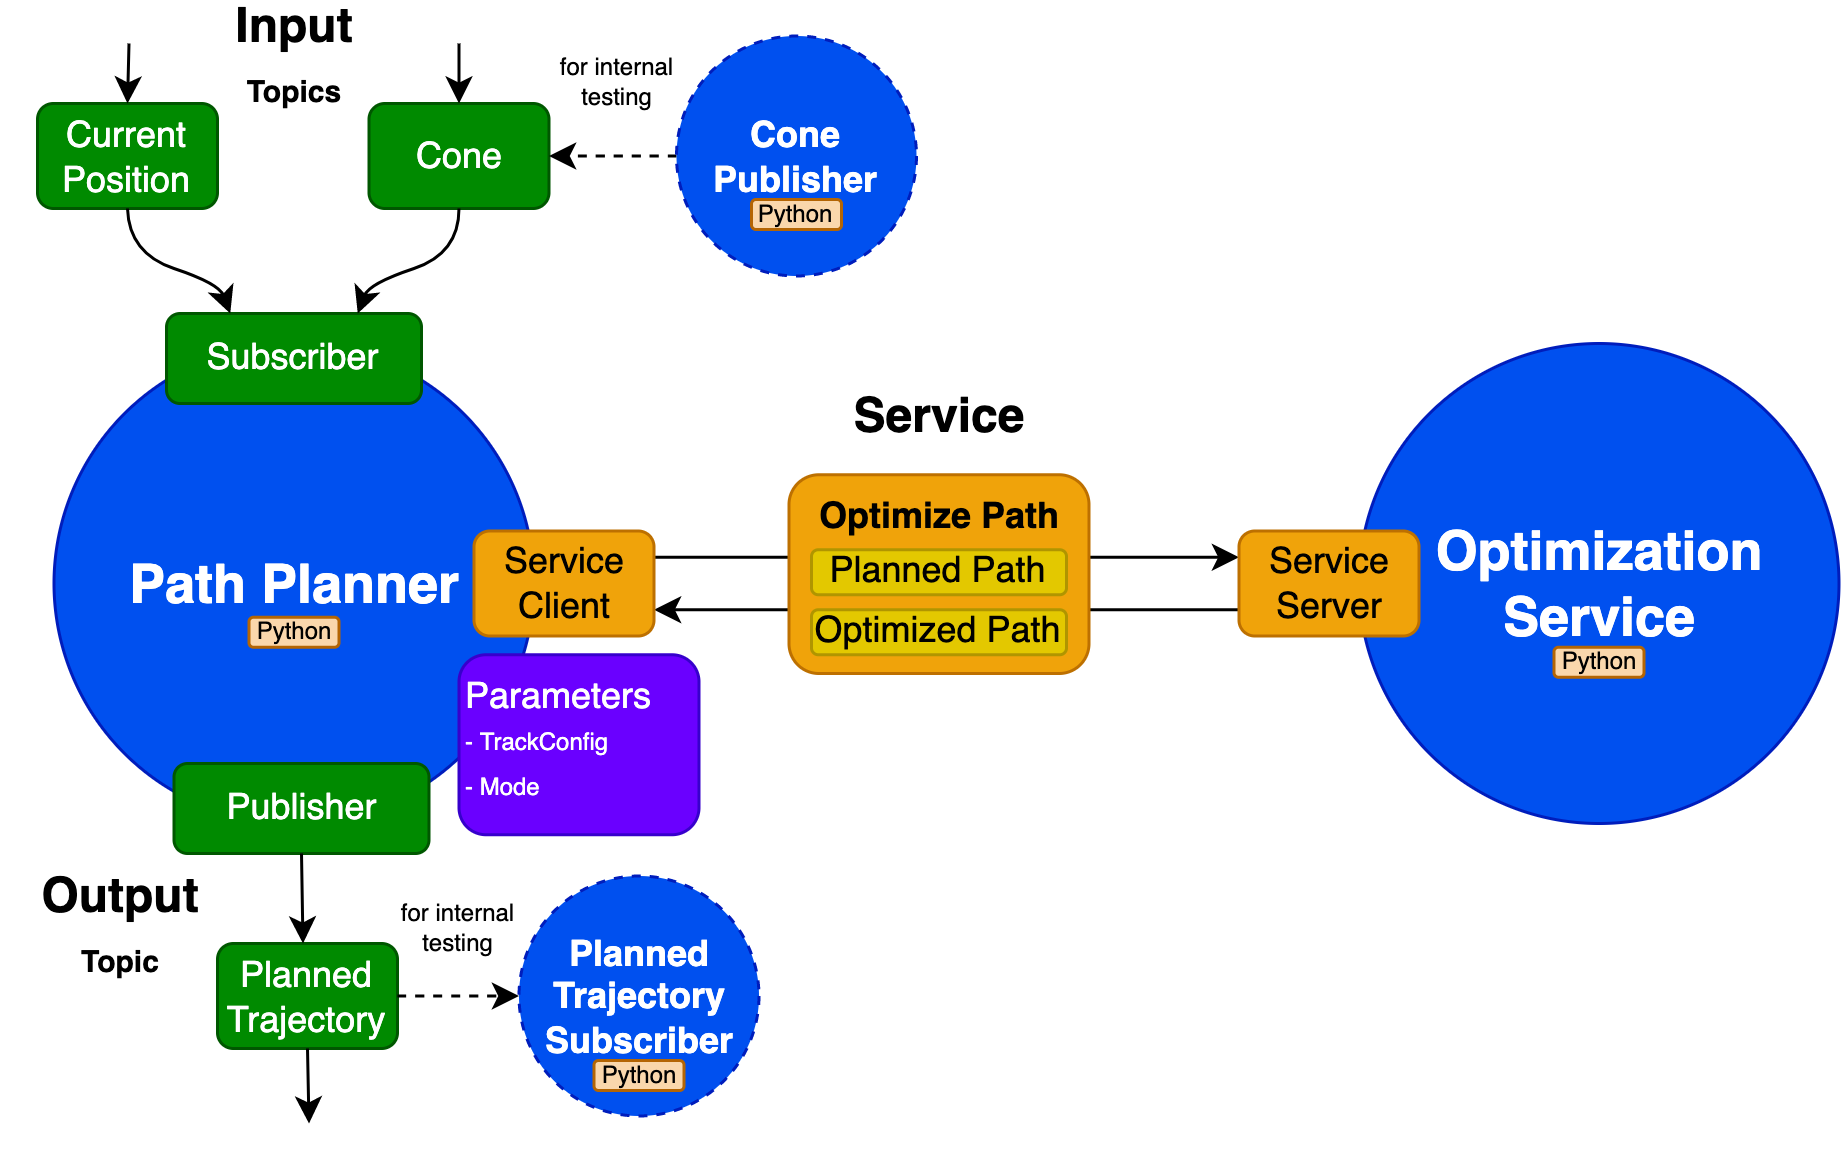
\includegraphics[width=\columnwidth]{Path_Planning_ROS_Architecture.png}
    \caption{The high-level ROS overview of the path planning package, consisting of several nodes and takes advantage of topics and services.}
    \label{fig:Path Planning ROS Architecture}
\end{figure}

The Path Planner node can be seen as the planner's brain, as it handles both the flow of the data and the management of the different algorithms. It subscribes to the inputs and publishes the output via \acrshort{ros} topics. While the 'Current Position' topic receives the car's current position, the 'Cone' topic receives the latest detected cone. The final planned path is then published via the 'Planned Trajectory' topic. The planner will calculate the path for the vehicle using the custom made 'Exploration Algorithm', which will be explained in more detail in section \ref{sec:Exploration Algorithm}. Furthermore, the node holds several configuration parameters regarding the algorithm mode, track configuration, and more.

The Path Planner requests the calculation of the optimized path to the Optimization Service. Communication with the service occurs through the 'Optimize Path' \acrshort{ros} service. While the Optimization Service calculates the optimized racing line for the given track, the Path Planner will continue to calculate the path using the exploration algorithm. The Path Planner will switch to publishing the optimized path after receiving the service's response.

For testing the package locally in Python, two additional \acrshort{ros} nodes were created: The 'Cone Publisher', for mocking the publishing of cones, and the 'Planned Trajectory Subscriber', for receiving the published trajectories by the planner. The verification steps are later described in section \ref{sec:Verification}.

\subsection{Custom ROS Messages} \label{sec:Custom ROS Messages}
As seen in section \ref{sec:Zurich UAS Racing Autonomous System}, for the Autonomous System to fully function, different components developed by different people will have to work together. Smooth communication between these different components is achieved via a set of default \acrshort{ros} messages defined by the team as seen in figure \ref{fig:Path Planning ROS Messages}. For \acrshort{ros} communication inside the Path Planning component itself, another package containing \acrshort{ros} messages was created. These messages are used between the topics and services seen in figure \ref{fig:Path Planning ROS Architecture}.

While the 'interfaces' package contains path planning internal ROS messages, the 'fszhaw\_msgs' package contains the messages for communication with the rest of the system. The 'OptimizePath.srv' message is used by the 'optimize\_path' service for the communication between the Path Planner and the Optimization Service, as seen in figure \ref{fig:Path Planning ROS Architecture}. From the 'fszhaw\_msgs' package, following messages are used in the Path Planning component: 'Cone.msg' for the 'cone' topic, 'CurrentPosition.msg' for the 'current\_position' topic, 'PlannedTrajectory.msg' for the 'planned\_trajectory' topic, and 'Track.msg' for the 'testing\_only/track' topic used in combination with the Simulation Tool.

\begin{figure}[H]
    \centering
    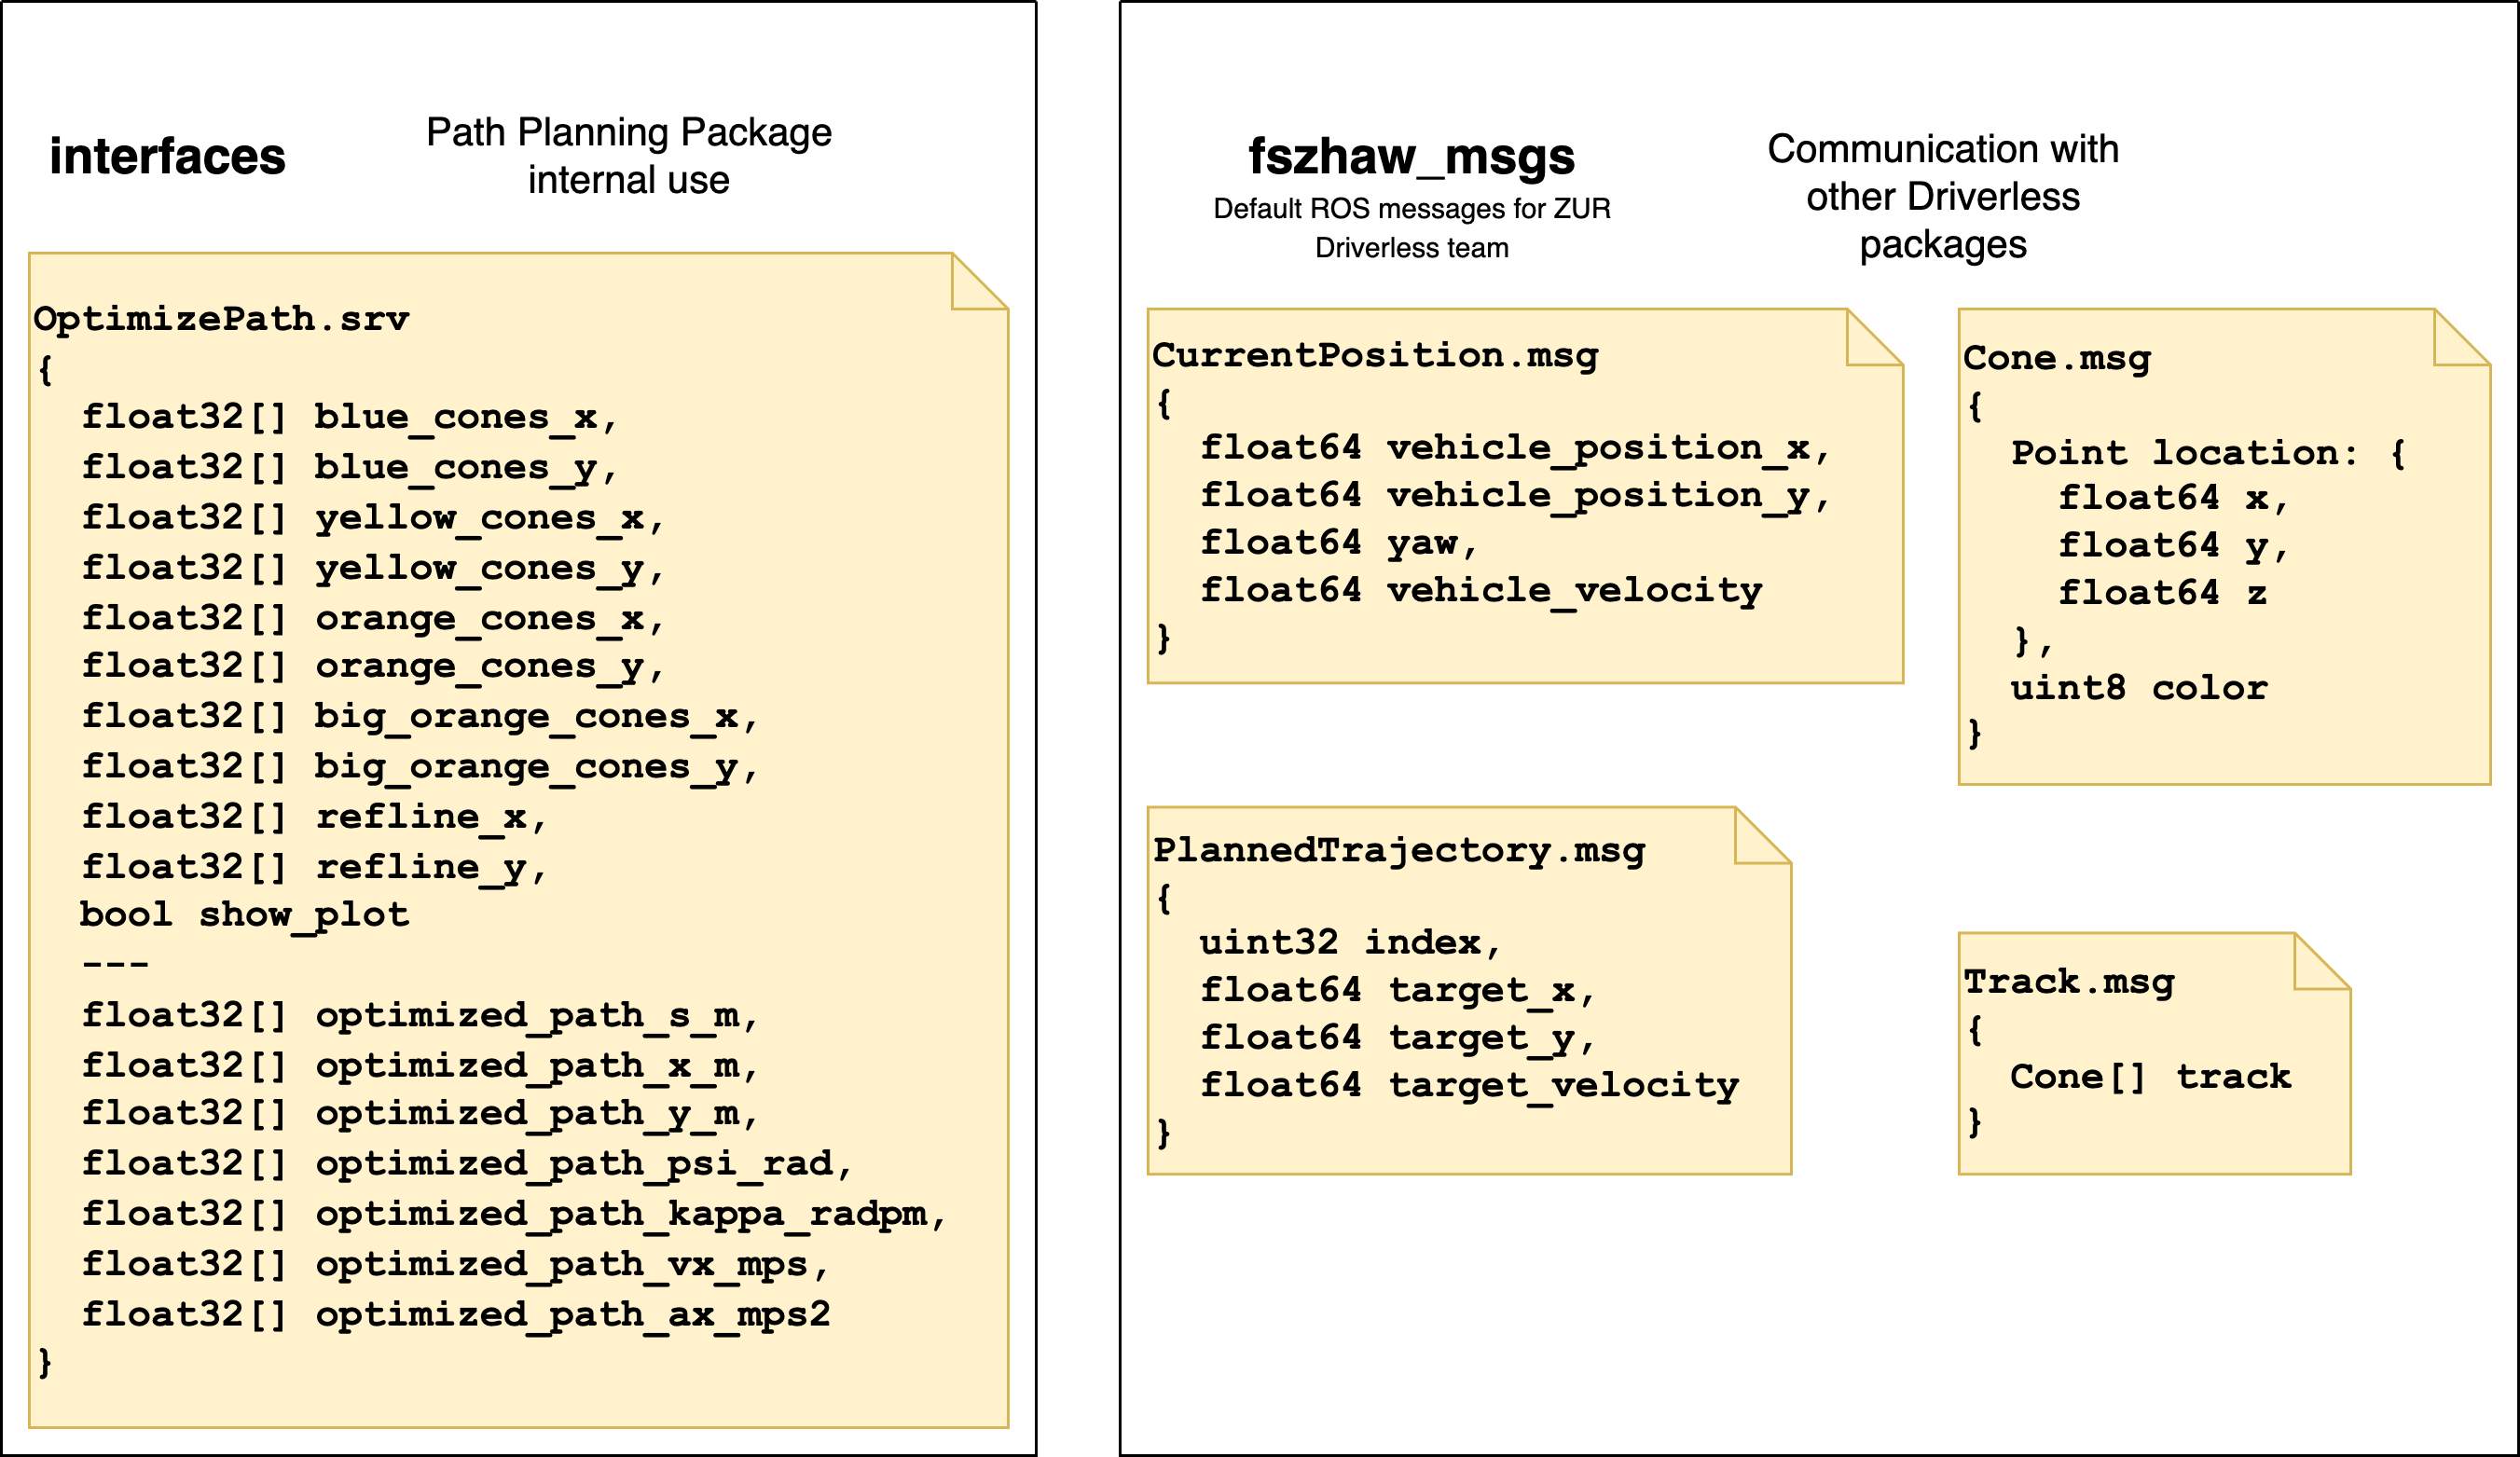
\includegraphics[width=\columnwidth]{Path_Planning_ROS_Messages.png}
    \caption{While the custom \acrshort{ros} messages in the 'interfaces' package are only used in the path planning package internally, the messages in the 'fszhaw\_msgs' package are used to communicate with the other packages in the autonomous system. These messages are used for the topics and services as seen in the \acrshort{ros} architecture in figure \ref{fig:Path Planning ROS Architecture}.}
    \label{fig:Path Planning ROS Messages}
\end{figure}

\subsection{Path Planner Node} \label{sec:Path Planner Node}
As seen in the component architecture of the Path Planning package in figure \ref{fig:Path Planning ROS Architecture}, the Path Planner node is the central processor of the whole package.
While receiving the detected cones and current position by the subscribers, the 'Start Finish Detector' can discern if the vehicle has reached the start of the track again. If not, the planner will calculate the planned path using the Exploration Algorithm and output it via the publisher. If a full lap has been completed, the planner will send a request for optimization to the 'Optimization Service'. After receiving the optimized path, it will send that via the publisher instead of the path calculated by the Exploration Algorithm. An overview of the Path Planner Node can be seen in figure \ref{fig:Path Planning Path Planner Node}.
\begin{figure}[H]
    \centering
    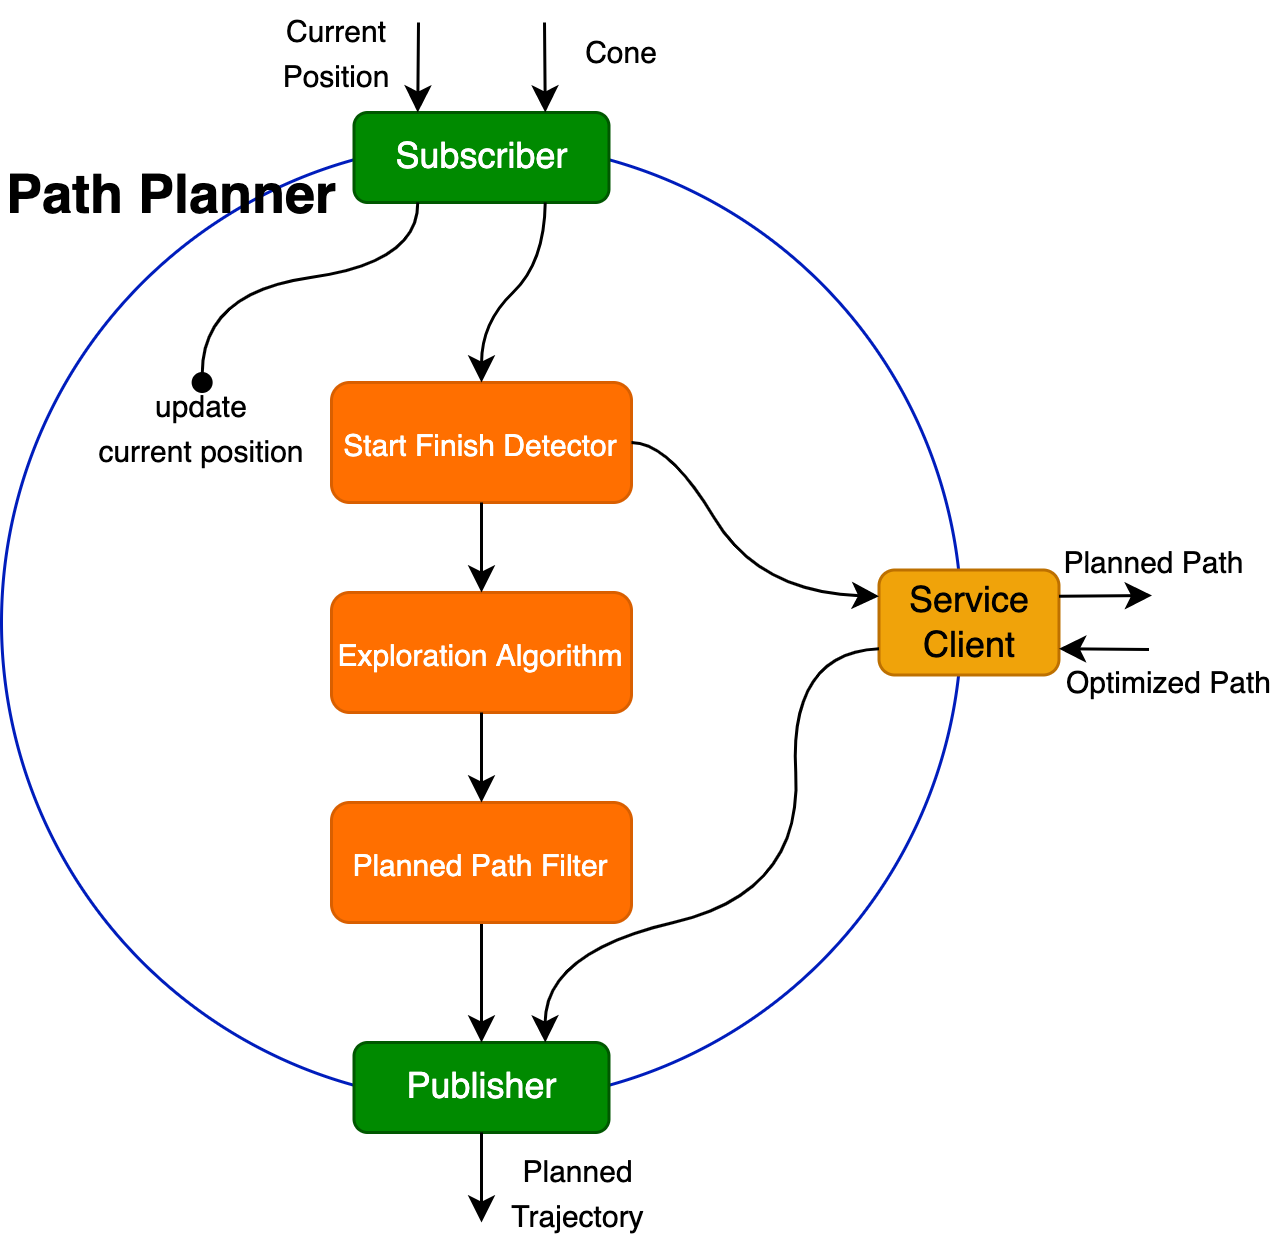
\includegraphics[width=10cm]{Path_Planning_Path_Planner.png}
    \caption{The same Path Planner Node as seen in figure \ref{fig:Path Planning ROS Architecture}, but in more detail. The Path Planner Node is made up of several components, a component for detecting the start of the track, the Exploration algorithm itself, a component for filtering which path points are published, and the \acrshort{ros} subscriber, publisher and service client.}
    \label{fig:Path Planning Path Planner Node}
\end{figure}

\subsubsection{Start Finish Detector} \label{sec:Start Finish Detector} %TODO mit welchem Theorieteil hat es einen Zusammenhang?
The 'Start Finish Detector' is responsible for realizing when the start or the track's end has been reached. There are two different ways the detector detects such a finish: By comparing its current position with the initial starting position or by detecting several big orange cones, which mark the starting line of a lap.

For events where the tracks are fully enclosed circuits, the end of a lap can be detected by just comparing the car's current position with the initial starting position at the beginning of the event, as illustrated in figure \ref{fig:Path Planner Start Finish Detector 1 and 2}.
\begin{figure}[H]
    \centering
    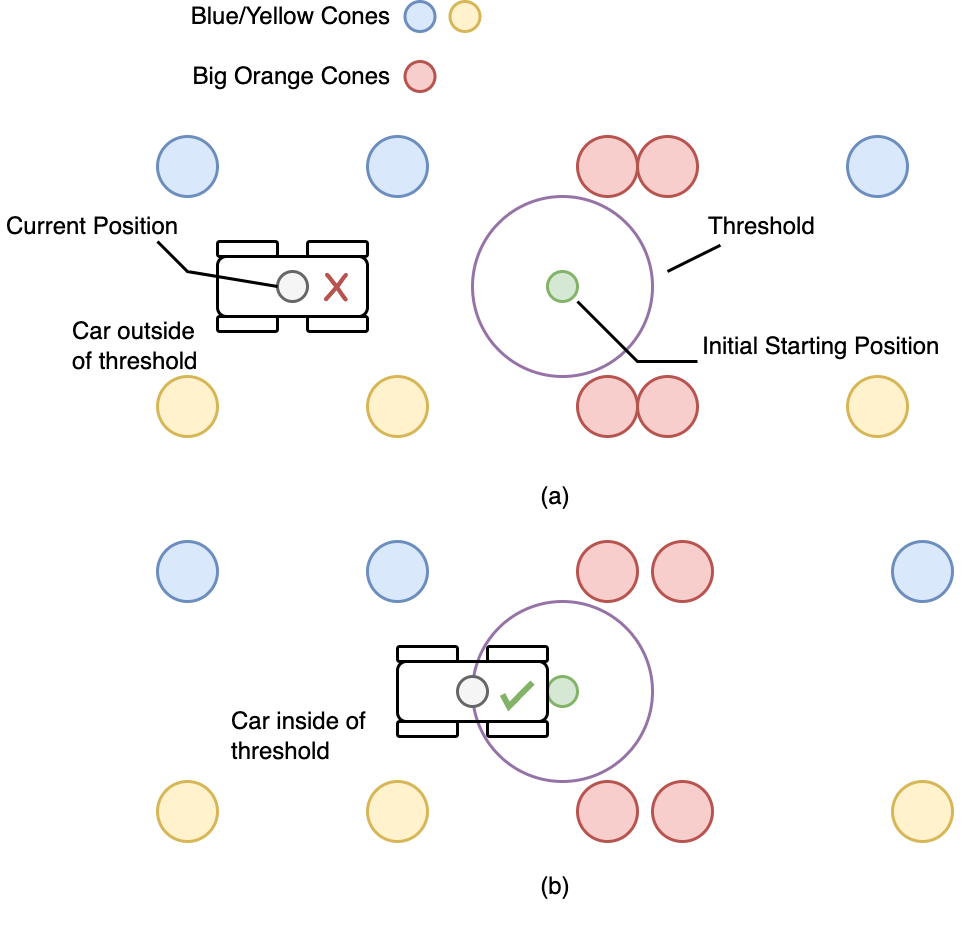
\includegraphics[width=\columnwidth]{Path_Planner_Start_Finish_Detector_1_2.png}
    \caption{In figure (a), a full lap will not be detected until the car reaches the threshold surrounding the initial starting position. In figure (b), the component will detect the completion of the lap as soon as the car reaches the threshold surrounding the initial starting position.}
    \label{fig:Path Planner Start Finish Detector 1 and 2}
\end{figure}

For events where the initial starting position is not the start respectively the end of a track, as with the Acceleration or Skidpad event, the starting line needs to be detected by encountering big orange cones, which mark the end of a track. These detected cones need to be close enough to be counted as a valid start/finish cone, or else they will be ignored, as seen in figure \ref{fig:Path Planner Start Finish Detector 3}.
\begin{figure}[H]
    \centering
    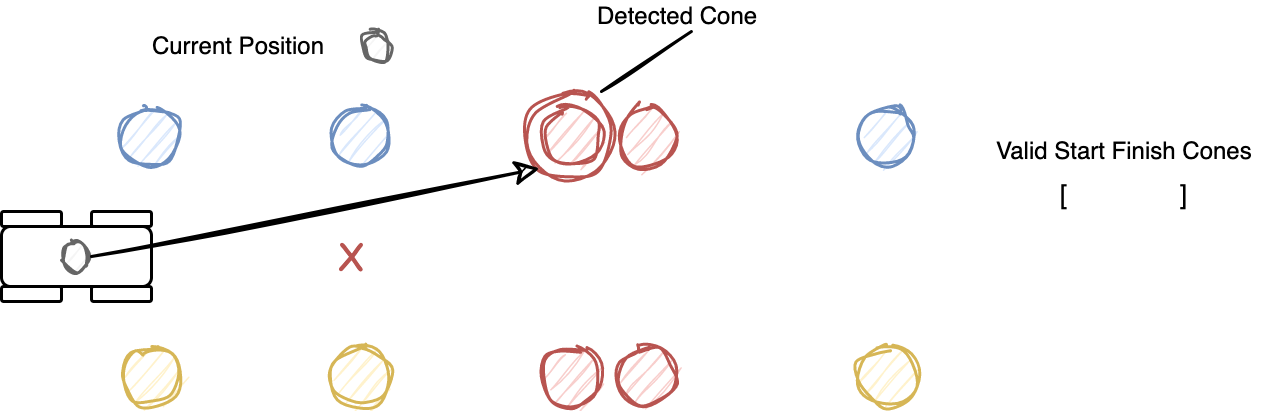
\includegraphics[width=\columnwidth]{Path_Planner_Start_Finish_Detector_3.png}
    \caption{The cone will be disregarded, as it is outside the threshold distance.}
    \label{fig:Path Planner Start Finish Detector 3}
\end{figure}
As soon as a big orange cone gets detected inside the threshold, it will be added as a valid start/finish cone, as shown in figure \ref{fig:Path Planner Start Finish Detector 4}
\begin{figure}[H]
    \centering
    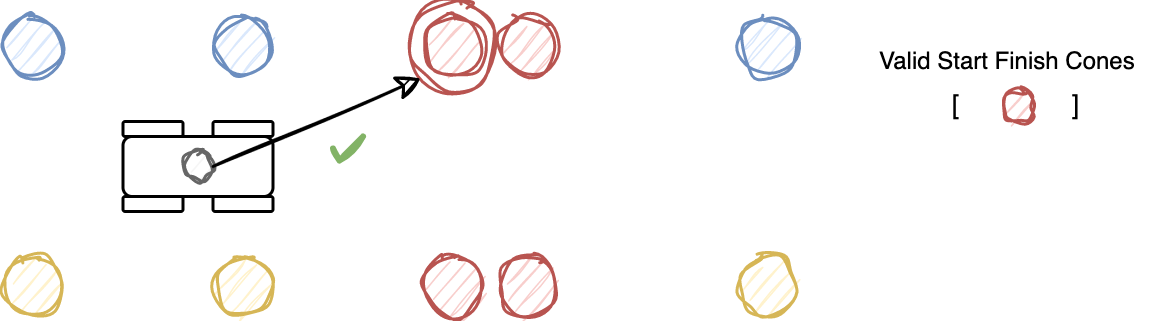
\includegraphics[width=\columnwidth]{Path_Planner_Start_Finish_Detector_4.png}
    \caption{The cone will be added as a valid start/finish cone, as its distance is inside the threshold.}
    \label{fig:Path Planner Start Finish Detector 4}
\end{figure}
After enough valid start/finish cones get added, e.g. two cones, will the detector check the distances between the added cones to see if they are really in the same area. If so, will the class successfully detect the completion of the track, as shown in figure \ref{fig:Path Planner Start Finish Detector 5}.
\begin{figure}[H]
    \centering
    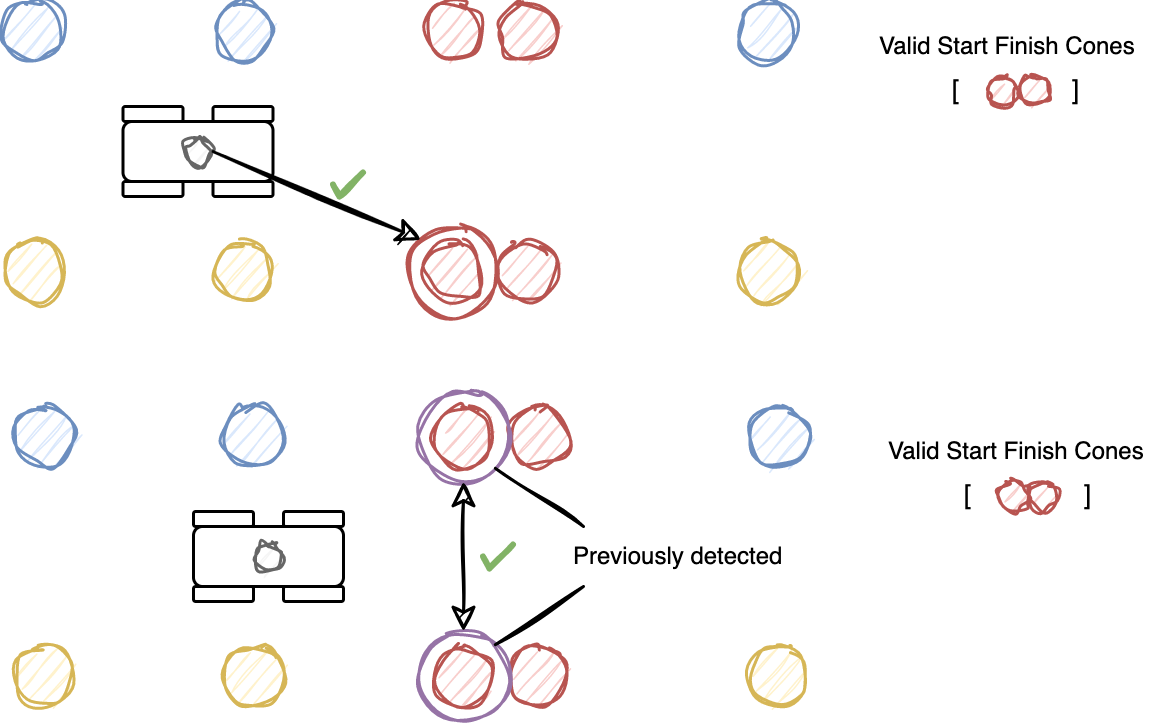
\includegraphics[width=\columnwidth]{Path_Planner_Start_Finish_Detector_5.png}
    \caption{Two valid start/finish cones get added, and the completion of the track is successfully detected.}
    \label{fig:Path Planner Start Finish Detector 5}
\end{figure}

\subsubsection{Exploration Algorithm} \label{sec:Exploration Algorithm} %TODO Zusammenhang mit Theorieteil?
The implementation of the exploration algorithm is found in the python file ``exploration/exploration.py'' inside the ``algorithm'' package. The algorithm uses several steps to get the middle line out of the cone's position and the car's position on the track. Figures \ref{fig:Algorithm Exploration Figure A} until \ref{fig:Algorithm Exploration Figure I, J and K} showcase the different steps of the algorithm. The algorithm only starts after two or more cones have been received from the ``cone\_publisher''. Step (a) in figure \ref{fig:Algorithm Exploration Figure A} shows five previously received cones, the current position of the car and the following received cone.
\begin{figure}[H]
    \centering
    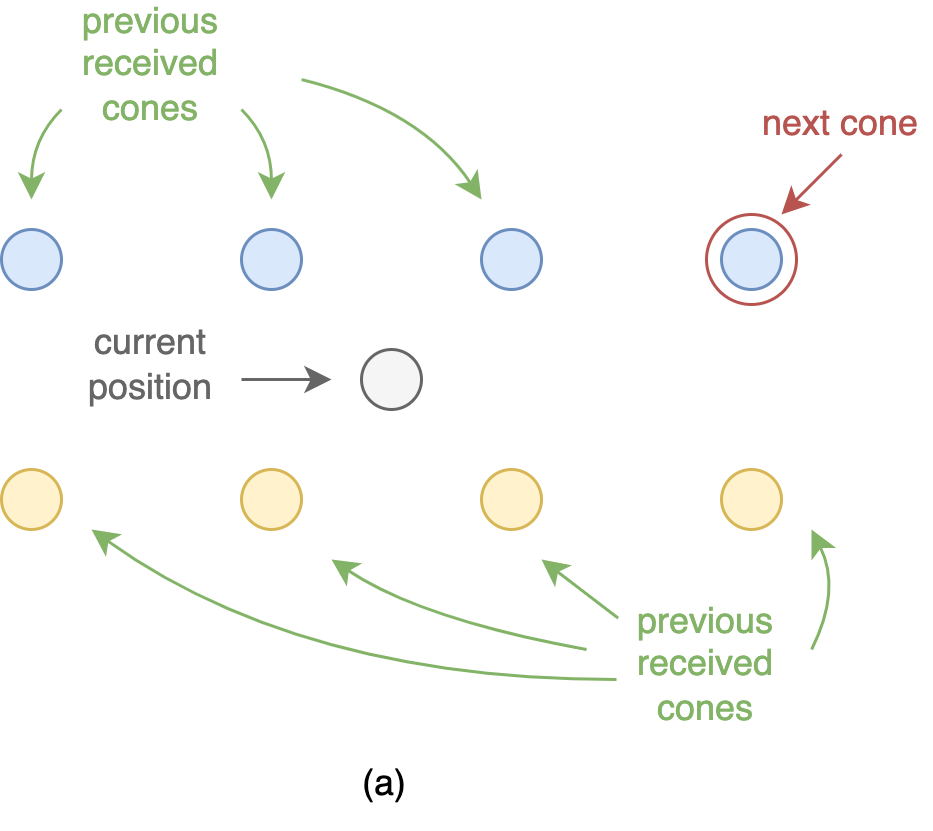
\includegraphics[width=8cm]{Algorithm_Exploration_Figure_A.png}
    \caption{In step (a), the next cone received is shown together with the previously received cones and the current position of the vehicle.}
    \label{fig:Algorithm Exploration Figure A}
\end{figure}

After having enough cones, the algorithm calculates the distance from the car to the newly received cone. It evaluates the distance based on a threshold which is defined in a track configuration file as shown in step (b) in figure \ref{fig:Algorithm Exploration Figure B and C}. If the distance is in the threshold, then new distances are calculated from the new cone to the previously received cones as shown in step (c) in figure \ref{fig:Algorithm Exploration Figure B and C}. These distances have a different threshold and evaluate if the previously received cones are suitable for triangulation.
\begin{figure}[H]
    \centering
    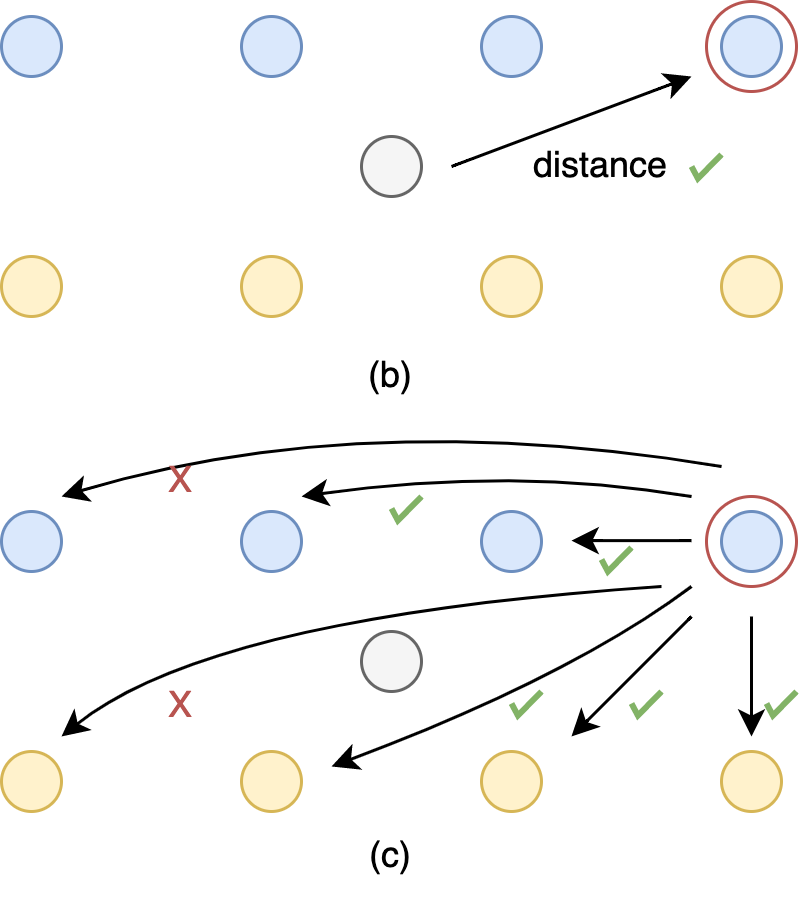
\includegraphics[width=8cm]{Algorithm_Exploration_Figure_B_C.png}
    \caption{Step (b) shows the calculation of the distance between the current position and the next received cone. Step (c) shows the distances between the newly received cones and the previously received cones. Cones inside a threshold will be used for triangulation.}
    \label{fig:Algorithm Exploration Figure B and C}
\end{figure}

Then the triangulation between the cones in the threshold and the new cone is calculated, as shown in step (d) in figure \ref{fig:Algorithm Exploration Figure D and E}. After the calculation of the triangles, simplices are evaluated between the cones as shown in step (e) in figure \ref{fig:Algorithm Exploration Figure D and E}. These simplices or triangles consist of several edges.
\begin{figure}[H]
    \centering
    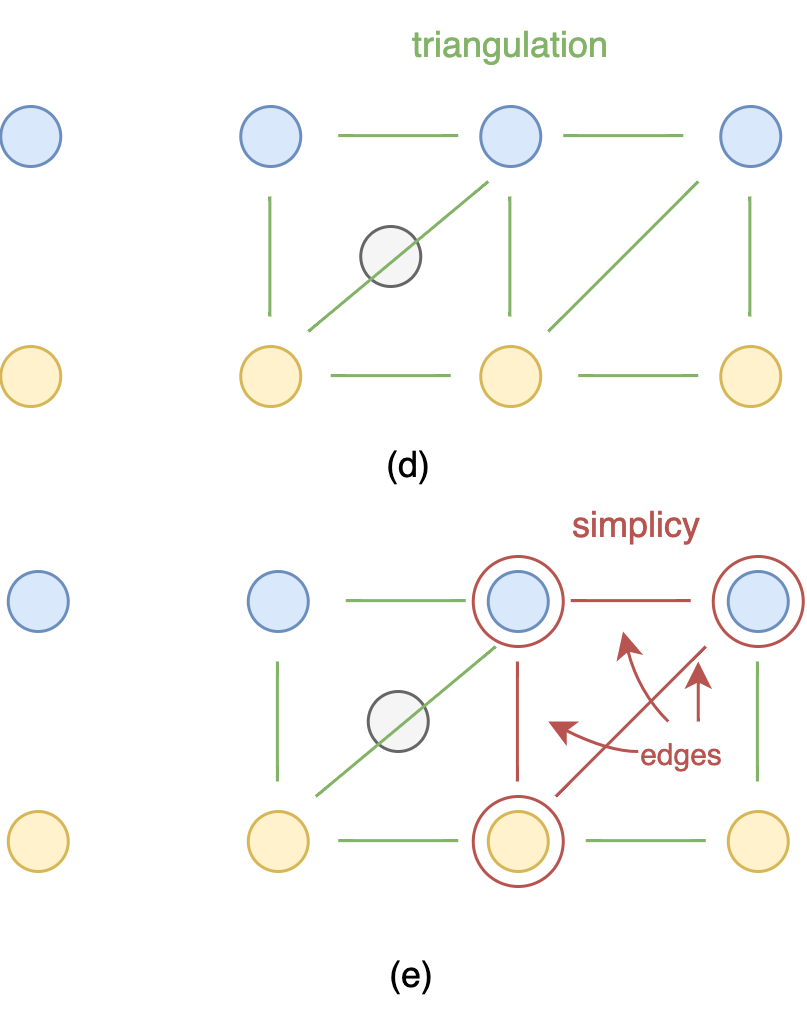
\includegraphics[width=8cm]{Algorithm_Exploration_Figure_D_E.png}
    \caption{In step (d), the triangulation between the cones is executed. In step (e), it can be seen that simplices have been created during the triangulation process, which themselves are made up of edges.}
    \label{fig:Algorithm Exploration Figure D and E}
\end{figure}

Based on the information on the edges between the new cones and cones in the given threshold, step (f) and (g) in figure \ref{fig:Algorithm Exploration Figure F, G and H} shows how valuable edges are validated. Edges with cones of the same colour are not usable. The second criterion is that the edge can not be too long, which becomes especially relevant in a curve on the track. This process of evaluation is repeated for every simplicy as shown in step (h) in figure \ref{fig:Algorithm Exploration Figure F, G and H}.
\begin{figure}[H]
    \centering
    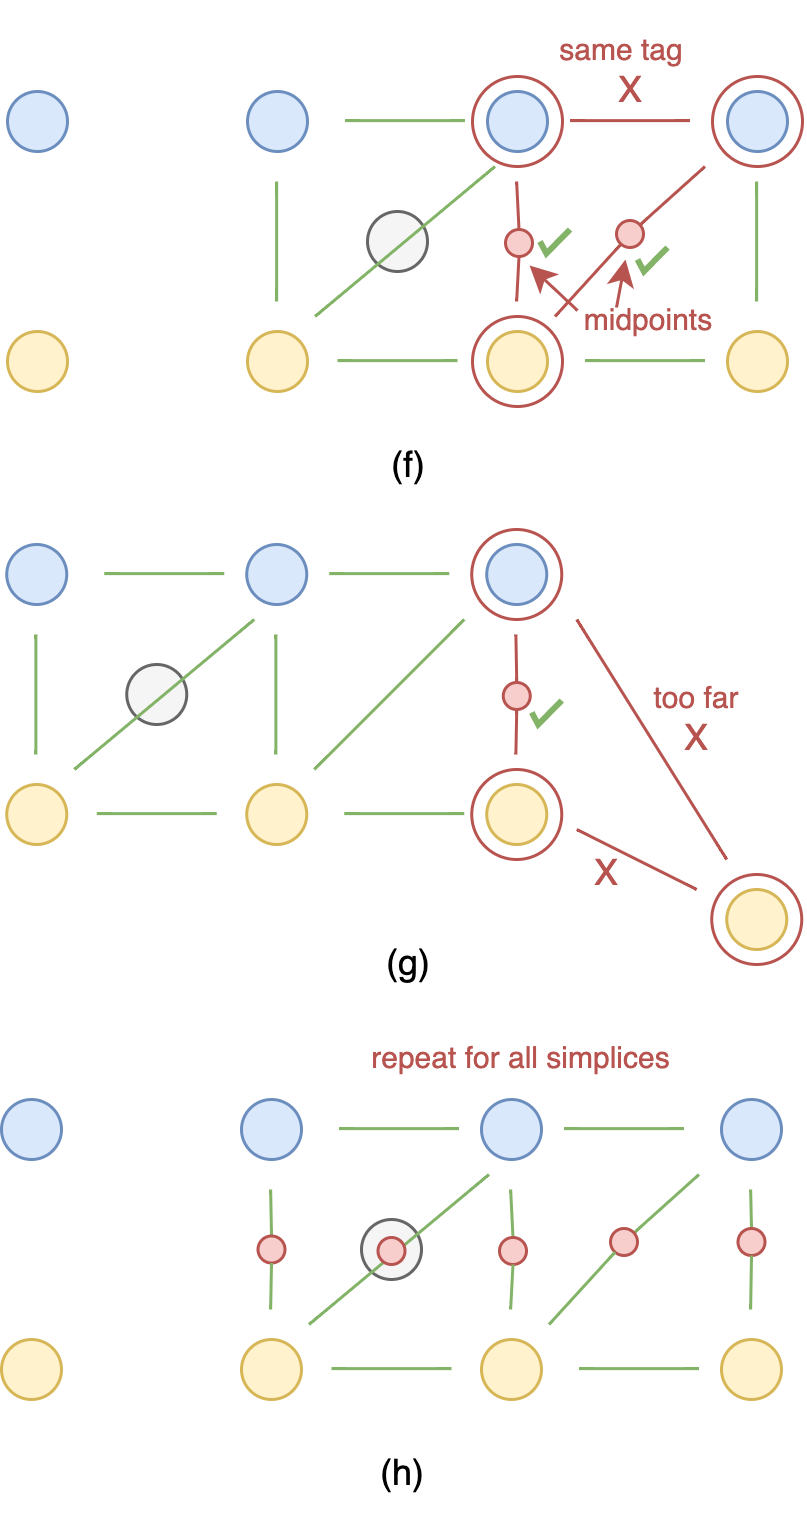
\includegraphics[width=8cm]{Algorithm_Exploration_Figure_F_G_H.png}
    \caption{Step (f) shows that edges with cones of the same colour are not used for the calculation of middle points. Step (g) shows that edges with a distance too long are also not considered for the calculation of middle points. In step (h), these checks will be made for every single simplicy created during triangulation.}
    \label{fig:Algorithm Exploration Figure F, G and H}
\end{figure}

The next step (i) is to build a path. Since the path is not smooth, spline interpolation is used to straighten the path in step (j), as seen in figure \ref{fig:Algorithm Exploration Figure I, J and K}. During Interpolation, the path will be densified, meaning the path will be added additional coordinates inside the interpolated path, as seen in step (k) in figure \ref{fig:Algorithm Exploration Figure I, J and K}. This path will then be published, and the optimization algorithm can use the generated points.
\begin{figure}[H]
    \centering
    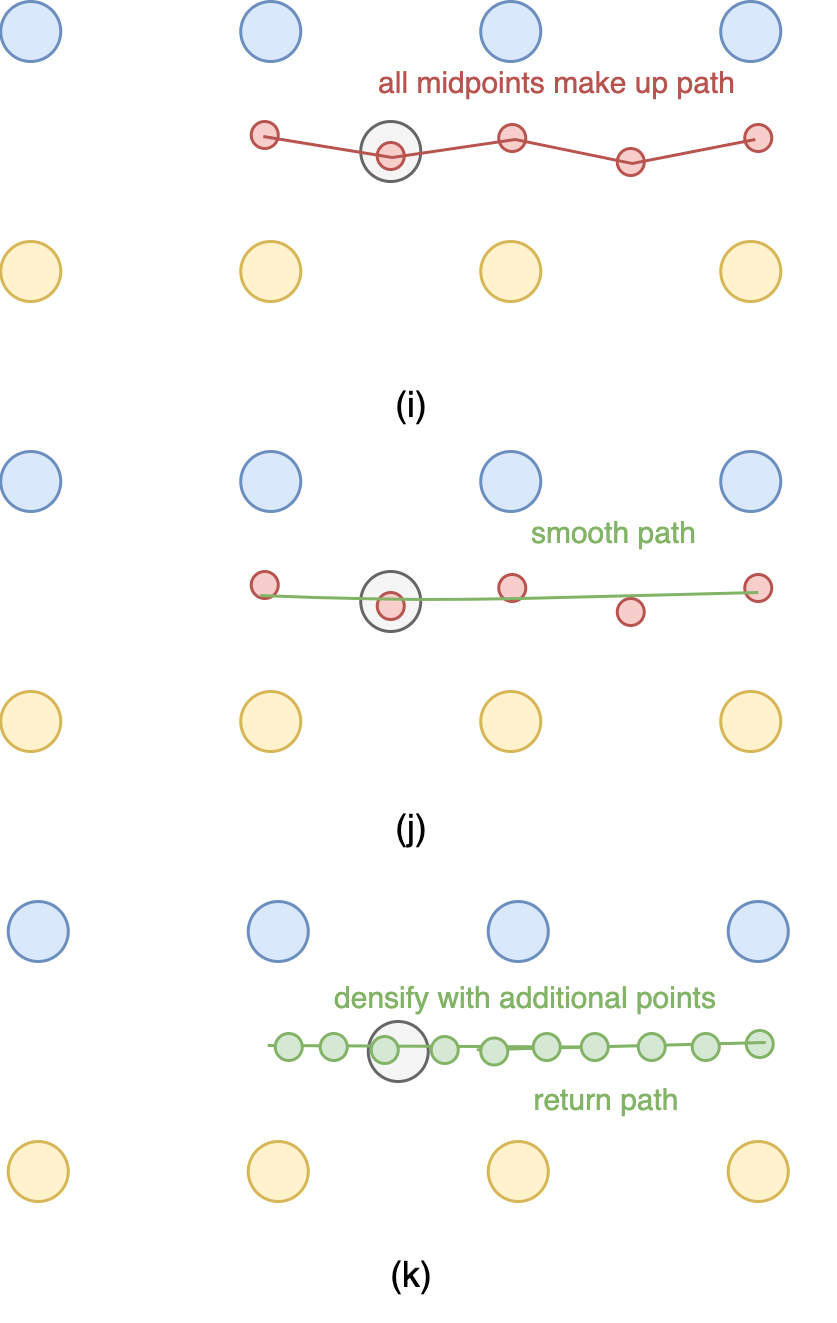
\includegraphics[width=8cm]{Algorithm_Exploration_Figure_I_J_K.png}
    \caption{Step (i) connects all processed middle points to a single path. Step (j) smooths that path using interpolation. Step (k) densifies the path during interpolation with additional path points.}
    \label{fig:Algorithm Exploration Figure I, J and K}
\end{figure}

The pseudocode of the exploration algorithm is shown in figure \ref{fig:Algorithm Exploration Pseudocode}. It starts with the distance from the car's current position to the new cone; the program checks if the distance is within the threshold. A list is created with all past cones at a reasonable distance to the new cone. The triangulation is calculated if the list is within the threshold of three or more cones. Further explanation is found in section \ref{sec:Motion Planning} under ``Combinatorial Motion Planning''. After the calculation of the simplices, the edges will be compared to each other so that no edges of the same ends are stored. After the comparison, another loop is undertaken to check if the cones on each edge do not have the same colour and are within the threshold. Each right edge will be added to the ``pathOfMiddlepoints'' array. After the program knows the potential middle points, a smoothening path algorithm is applied, followed by a densify algorithm to add more middle points. The algorithm then returns the final result containing the middle line.

\begin{figure}[H]
    \centering
    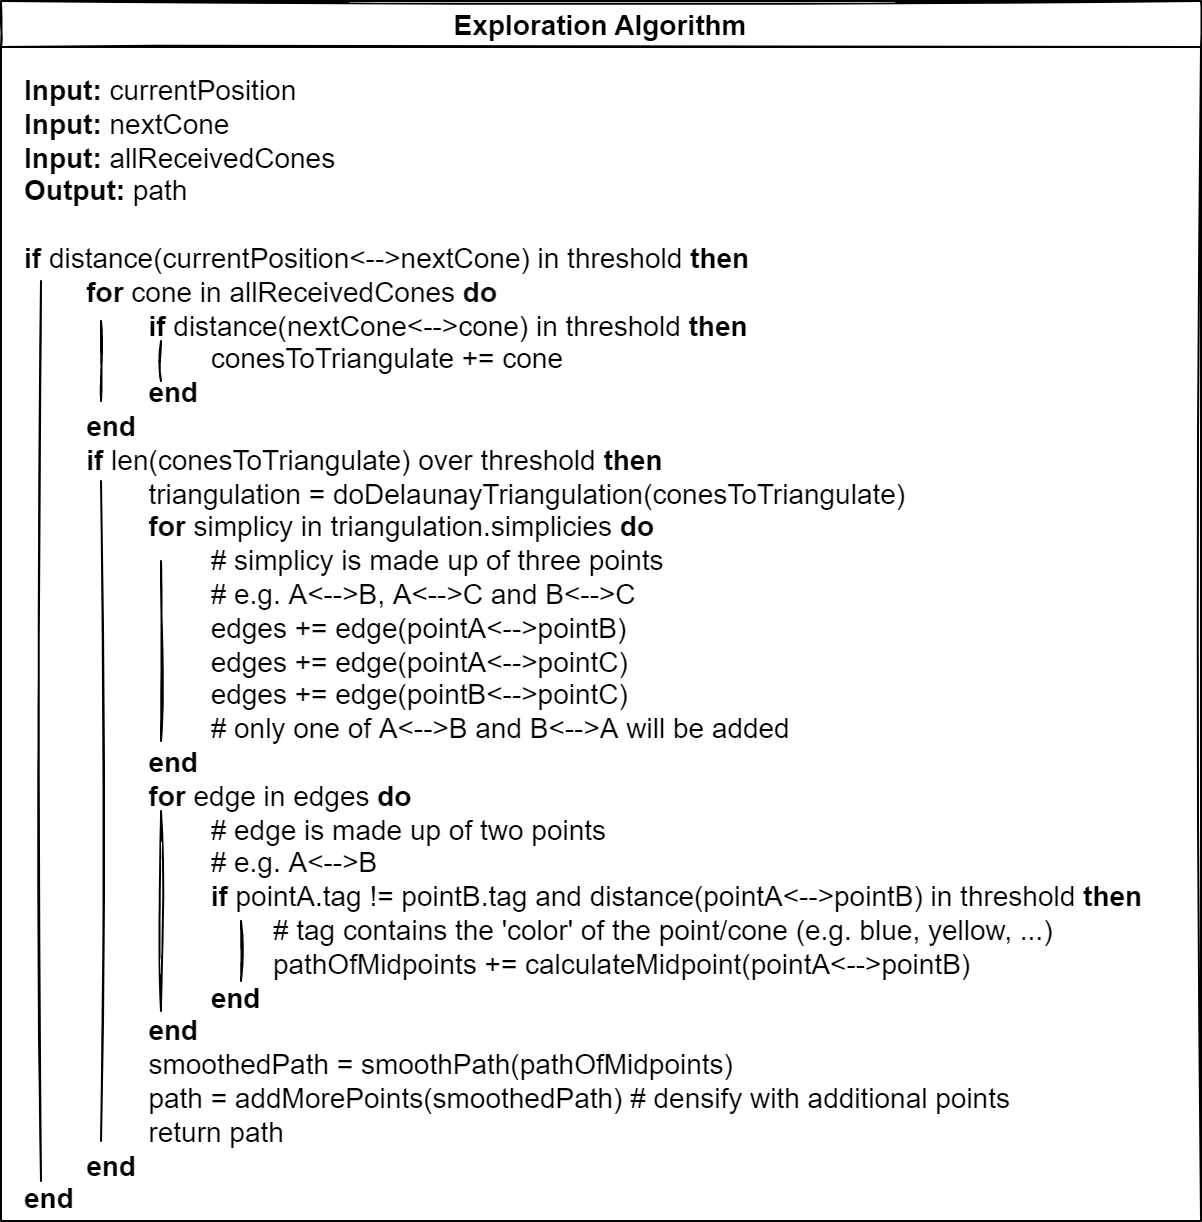
\includegraphics[width=12cm]{Algorithm_Exploration_Pseudocode.png}
    \caption{The exploration algorithm can be presented in a pseudocode program as well.}
    \label{fig:Algorithm Exploration Pseudocode}
\end{figure}

\subsubsection{Planned Path Filter} \label{sec:Planned Path Filter}
\lipsum[1]

\subsection{Optimization Service Node} \label{sec:Optimization Service Node}
As seen in the component architecture of the Path Planning package in figure \ref{fig:Path Planning ROS Architecture}, the Optimization Service Node is responsible for receiving the request for optimization by the Path Planner Node, preparing the input for optimization, optimizing the path, and then sending it back to the planner for further processing and publishing.

The node comprises two main components, the 'Optimization Input Transformer' and the 'Optimization Algorithm' itself. The node will receive all previously detected cones and a reference line of the driven track by the planner, e.g. the middle line. In this case, the reference line will be the calculated path by the 'Exploration Algorithm'. Because the 'Optimization Algorithm' expects a single reference line with its distances to the track's border as an input, a transformation of the received input is first needed before the algorithm can optimize it. With the data from all the received cones and reference line, the 'Optimization Input Transformer' can map the input to a single list of reference points and the distances from each point to the track's border. The transformer will be explained further in section \ref{sec:Optimization Input Transformer}. With that list, the 'Optimization Algorithm' can optimize the path concerning one of several objectives, e.g. the shortest path or minimum curvature. The algorithm will be explained in more detail in section \ref{sec:Optimization Algorithm}. The optimized path will then be sent back to the planner via the  \acrshort{ros} service.
\begin{figure}[H]
    \centering
    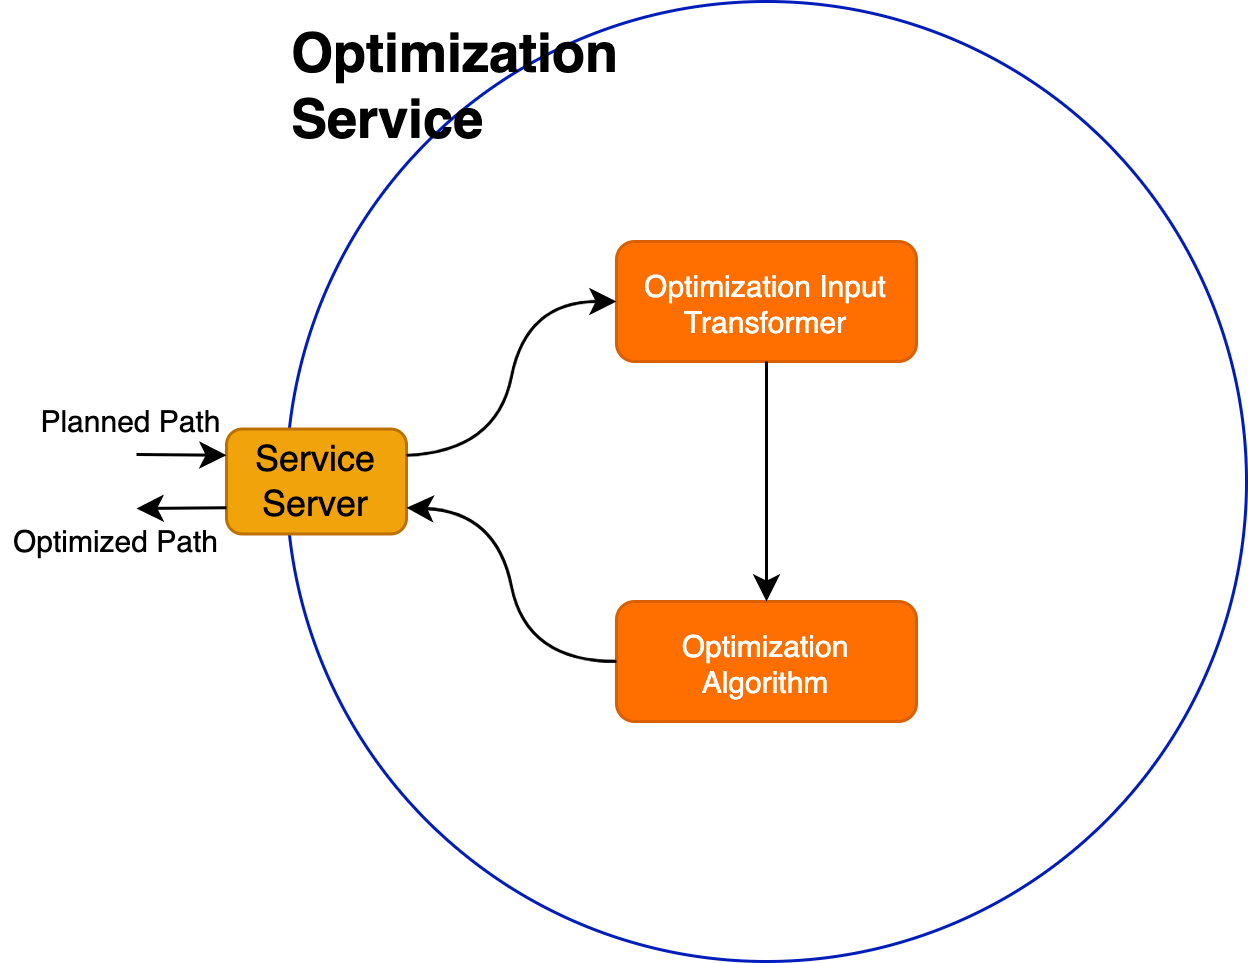
\includegraphics[width=10cm]{Path_Planning_Optimization_Service.png}
    \caption{The Optimization Service Node is made up of two main components, a component for preparing the received input for optimization and the algorithm to optimize the path itself.}
    \label{fig:Path Planning Optimization Service Node}
\end{figure}

\subsubsection{Optimization Input Transformer} \label{sec:Optimization Input Transformer}
As mentioned before in section \ref{sec:Optimization Service Node}, all previously detected cones (blue, yellow, orange and big orange cones) and a reference line, in this case, the calculated path by the Exploration Algorithm, are used as input by the Optimization Input Transformer. A newly created reference track consisting of reference points and their corresponding distances to the track's limits are received as the output. An illustration can be seen in figure \ref{fig:Optimization Service Input Transformer 1}
\begin{figure}[H]
    \centering
    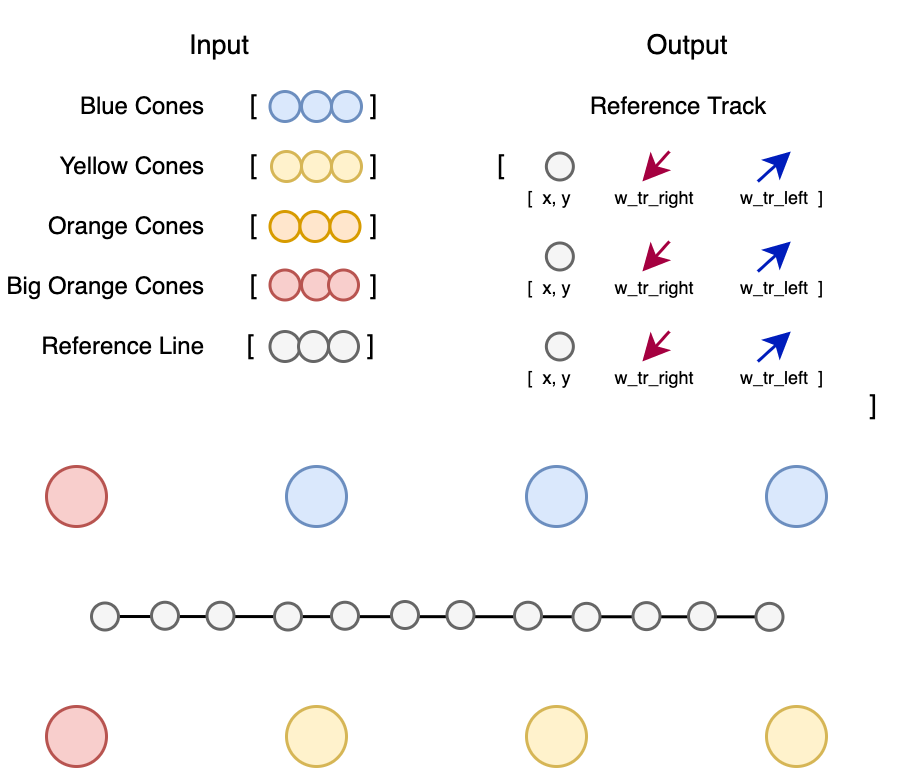
\includegraphics[width=10cm]{Optimization_Service_Input_Transformer_1.png}
    \caption{All previously received cones and a reference line are used as the input, while a reference track containing reference points and their distances to the track limits are received as the output.}
    \label{fig:Optimization Service Input Transformer 1}
\end{figure}
Firstly, the closest point on the reference line will be calculated for each given yellow or blue cone. For this step, the list with more cones will be chosen, e.g. the list with all yellow cones would be used if there are more yellow than blue cones. During this process, depending on the position of the orange and big orange cones, they will be classified as blue cones or as yellow cones.
\begin{figure}[H]
    \centering
    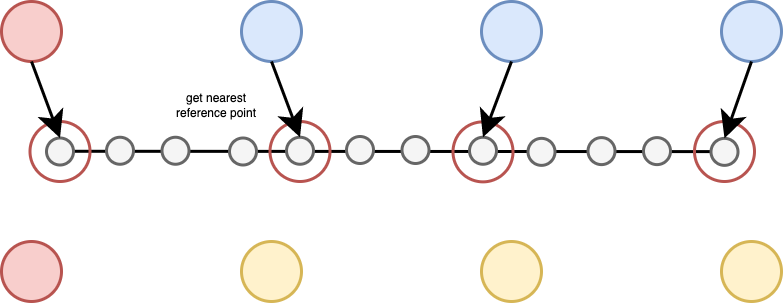
\includegraphics[width=10cm]{Optimization_Service_Input_Transformer_2.png}
    \caption{For each blue or yellow cone, its closest point on the reference line will be determined.}
    \label{fig:Optimization Service Input Transformer 2}
\end{figure}
Secondly, its distance to the track limits are calculated for each reference point. Because blue cones are always situated on the left side of the track, and yellow cones are always on the right side, the distance to the left track limit can be determined by computing the distance to its nearest blue cone. The right track limit can be determined by computing the distance to its nearest yellow cone.
\begin{figure}[H]
    \centering
    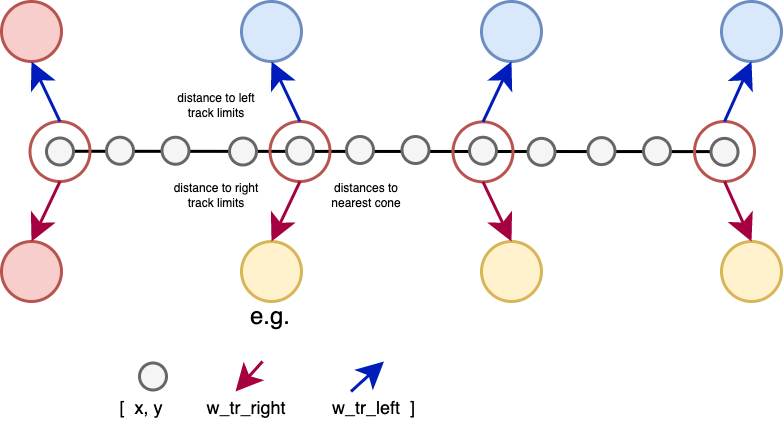
\includegraphics[width=10cm]{Optimization_Service_Input_Transformer_3.png}
    \caption{For each selected reference point, its distance to the left and right track limits will be computed, by just evaluating its distance to the nearest blue cone or yellow cone respectively.}
    \label{fig:Optimization Service Input Transformer 3}
\end{figure}
Lastly, the developed list containing the reference track will be returned as the output.

\subsubsection{Optimization Algorithm} \label{sec:Optimization Algorithm}
The base code of the implementation was forked from the Institute of Automotive Technology at the \acrlong{tum}.
The repository contains algorithms for determining an optimal racing line. It is possible to choose between several objectives: Shortest Path, Minimum Curvature (with or without iterative call) and Minimum Time (with or without powertrain behaviour consideration). \cite{tumftm_optimization_algoritm}

The racing line from the minimum curvature objective is quite near to a minimum time racing line in corners. However, it will differ when the car's acceleration limits are not exploited. However, the minimum time optimization requires more parameters and takes more computation time. It was decided to use the Minimum Curvature objective primarily, as the time difference between Minimum Curvature and Minimum Time is too small to justify its use over the other algorithms (see chapter \ref{ch:Results}). An overview of the whole optimization module is shown in figure \ref{fig:Optimization Algorithm Module Overview}.
\begin{figure}[H]
    \centering
    \includegraphics[width=\columnwidth]{Algorithm_Optimization_Module.png}
    \caption{The main method ``optimize\_path()'' inside the ``main\_globaltraj.py'' file (outlined green) imports parameters from the vehicle parameter file ``racecar.ini'' and receives its inputs, a reference track, an optional friction map and user configurations by the client. In the end, an optimal race trajectory line will be outputted.}
    \label{fig:Optimization Algorithm Module Overview}
\end{figure}

\textbf{Overview}

At the centre of the Optimization Algorithm is the main file called ``main\_globaltraj.py'', as it can be seen in figure \ref{fig:Optimization Algorithm Module Overview} (outlined green). A figure zoomed into the centre of the module can be seen in figure \ref{fig:Optimization Algorithm Module MainGlobalTraj}. This file includes the ``optimize\_path()'' function used to optimize the path. It imports various utility functions from the ``helper\_funcs\_glob'' package, it contains functions to import a reference track (``import\_track()''), to prepare the imported reference track for optimization (``prep\_track()'') or to plot resulting figures (``result\_plots()''), just to name a few. As a Python dependency, additional helper functions are imported from the ``trajectory\_planning\_helpers'' repository provided by \acrshort{tumftm}. \cite{tumftm_trajectory_planning_helpers}
These helpful helper functions for path and trajectory planning are frequently used in the trajectory planning software stack at \acrshort{tumftm}.
In the end, the most optimal race trajectory line will be outputted by the algorithm.
\begin{figure}[H]
    \centering
    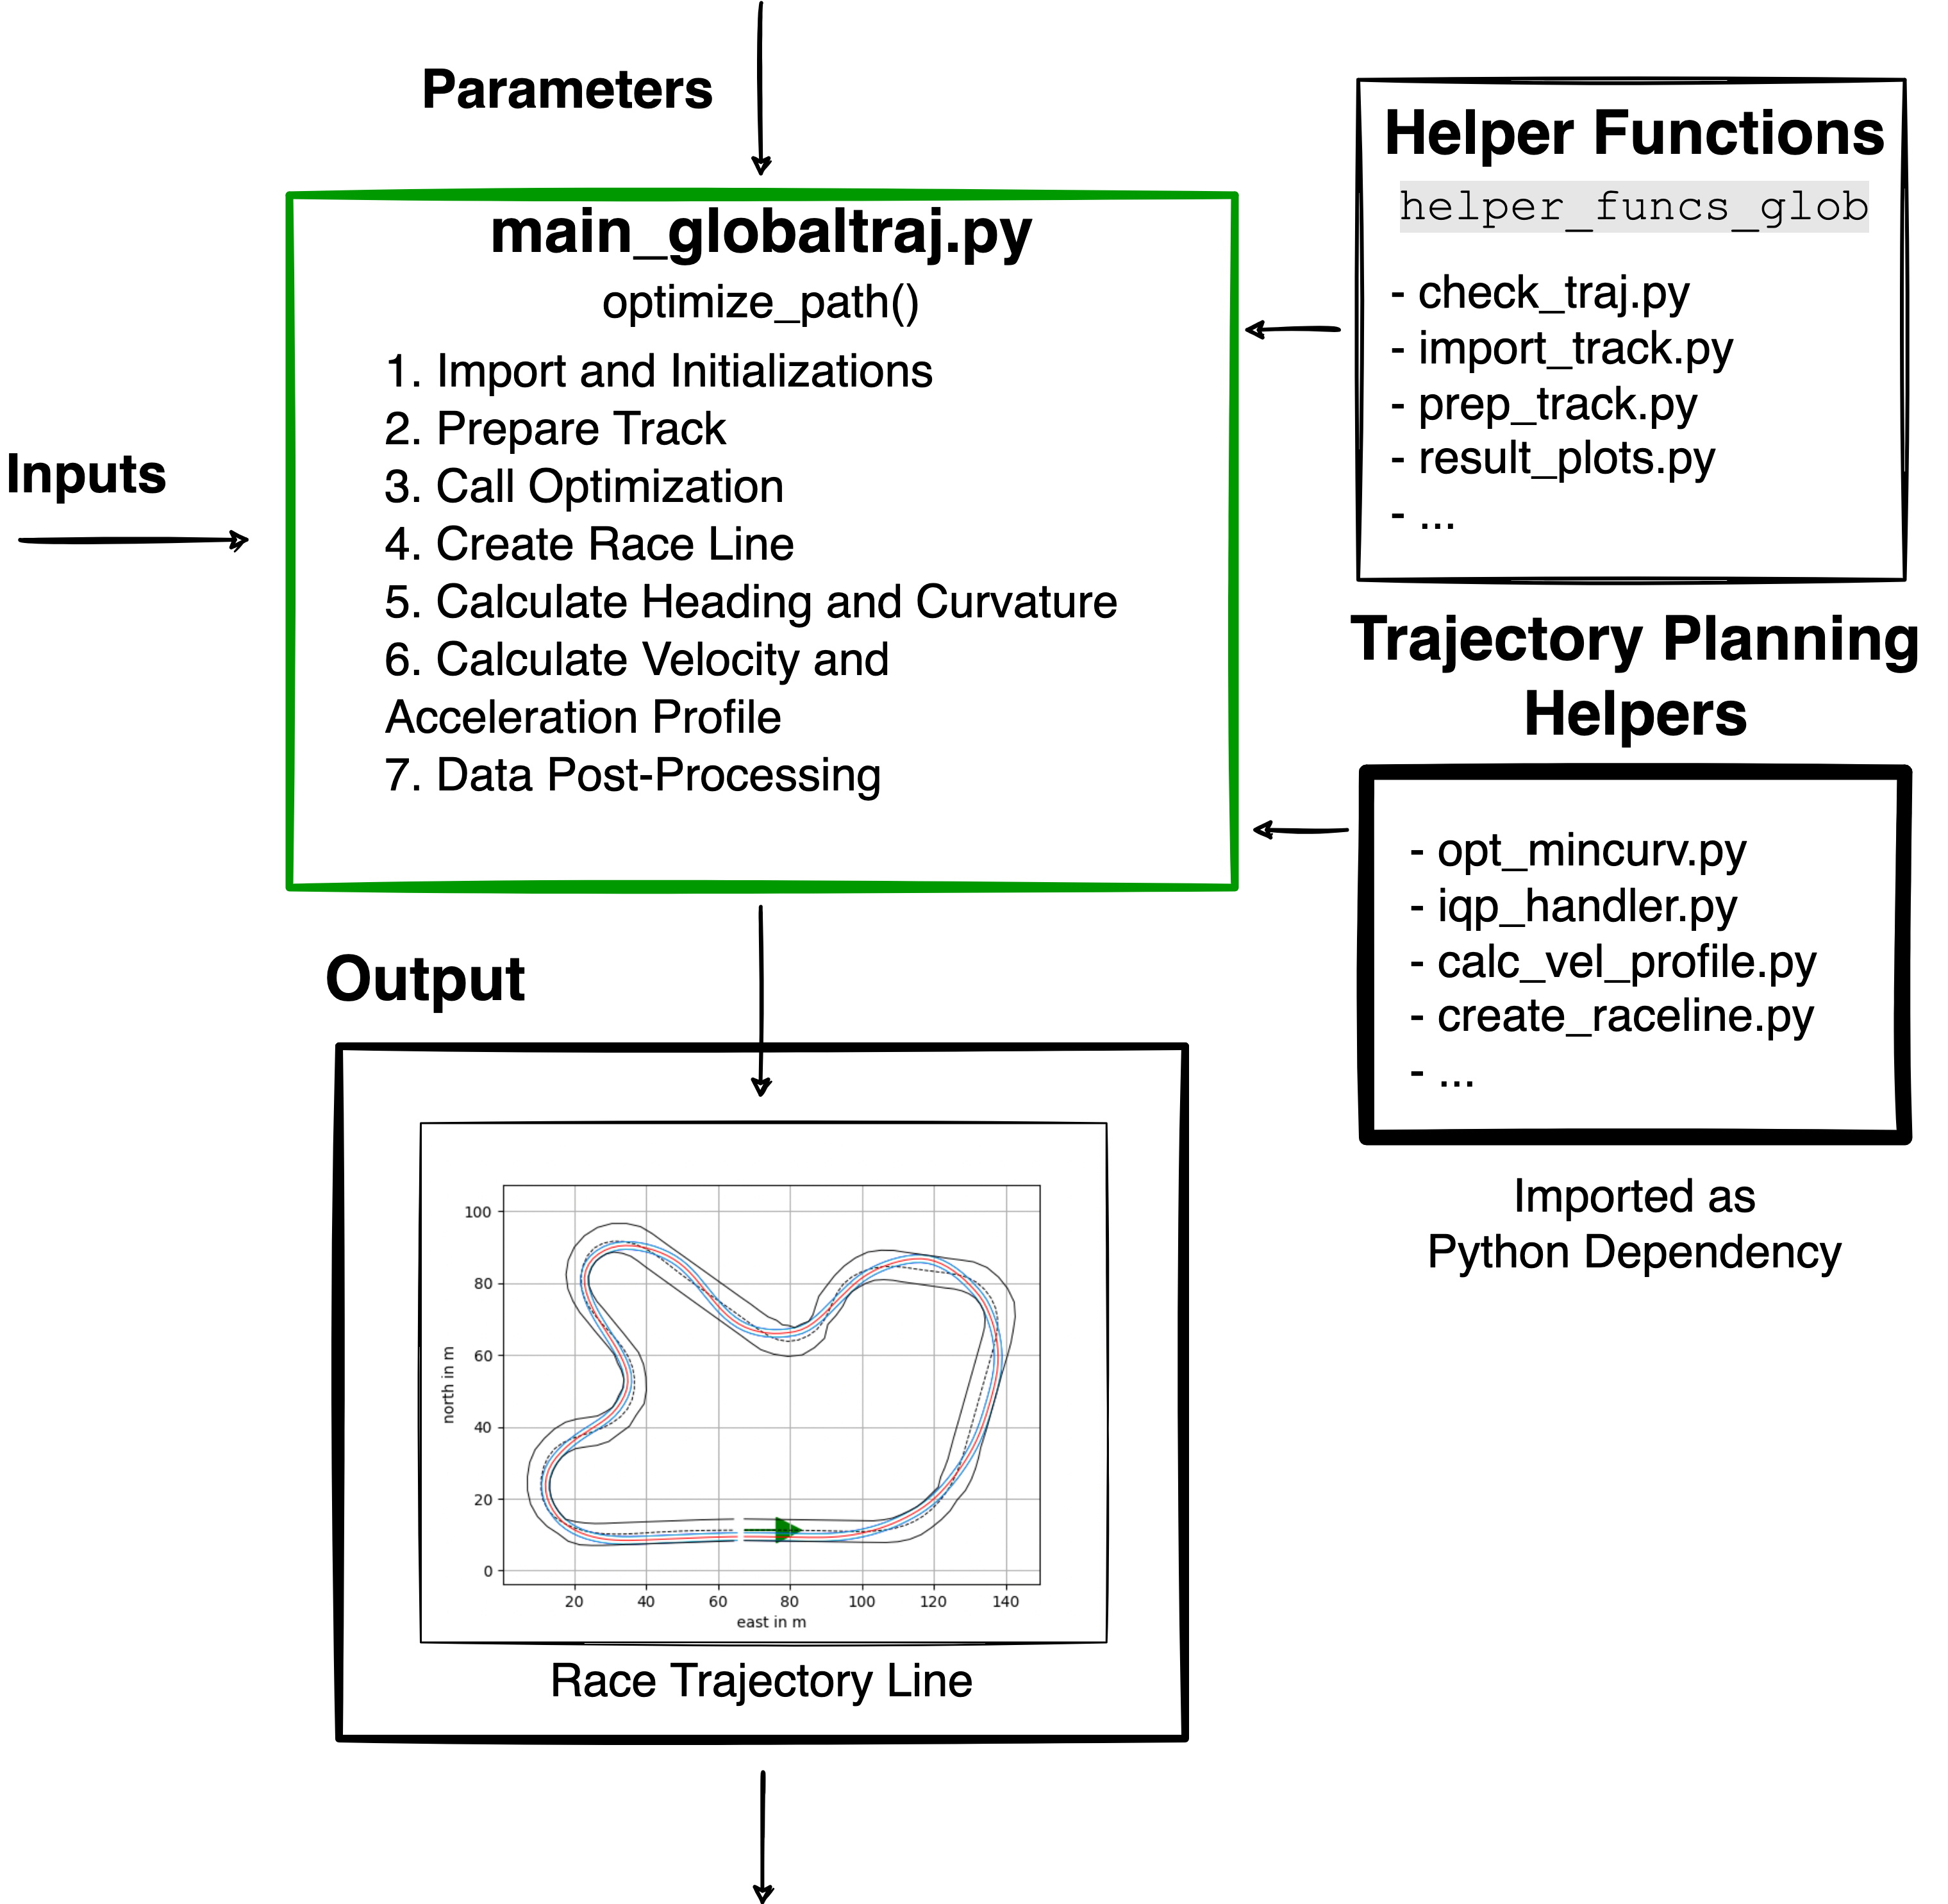
\includegraphics[width=\columnwidth]{Algorithm_Optimization_Module_MainGlobalTraj.png}
    \caption{The primary method of the project is located in main\_globaltraj.py and imports essential and useful functions from the helper\_funcs\_glob package and the external trajectory\_planning\_helpers repository. The output will be the calculated race trajectory line.}
    \label{fig:Optimization Algorithm Module MainGlobalTraj}
\end{figure}

\textbf{Inputs}

As for its inputs, the main method receives the required reference track and additional user configurations, like the optimization type, minimum track width, number of laps to be driven and more, by the client. A supplementary friction map of the track can also be provided but is only relevant for Minimum Time solutions. In principle, they can also be considered within the velocity profile calculation of Minimum Curvature solutions. However, this is currently not supported in this implementation. \cite{tumftm_optimization_algoritm}
\begin{figure}[H]
    \centering
    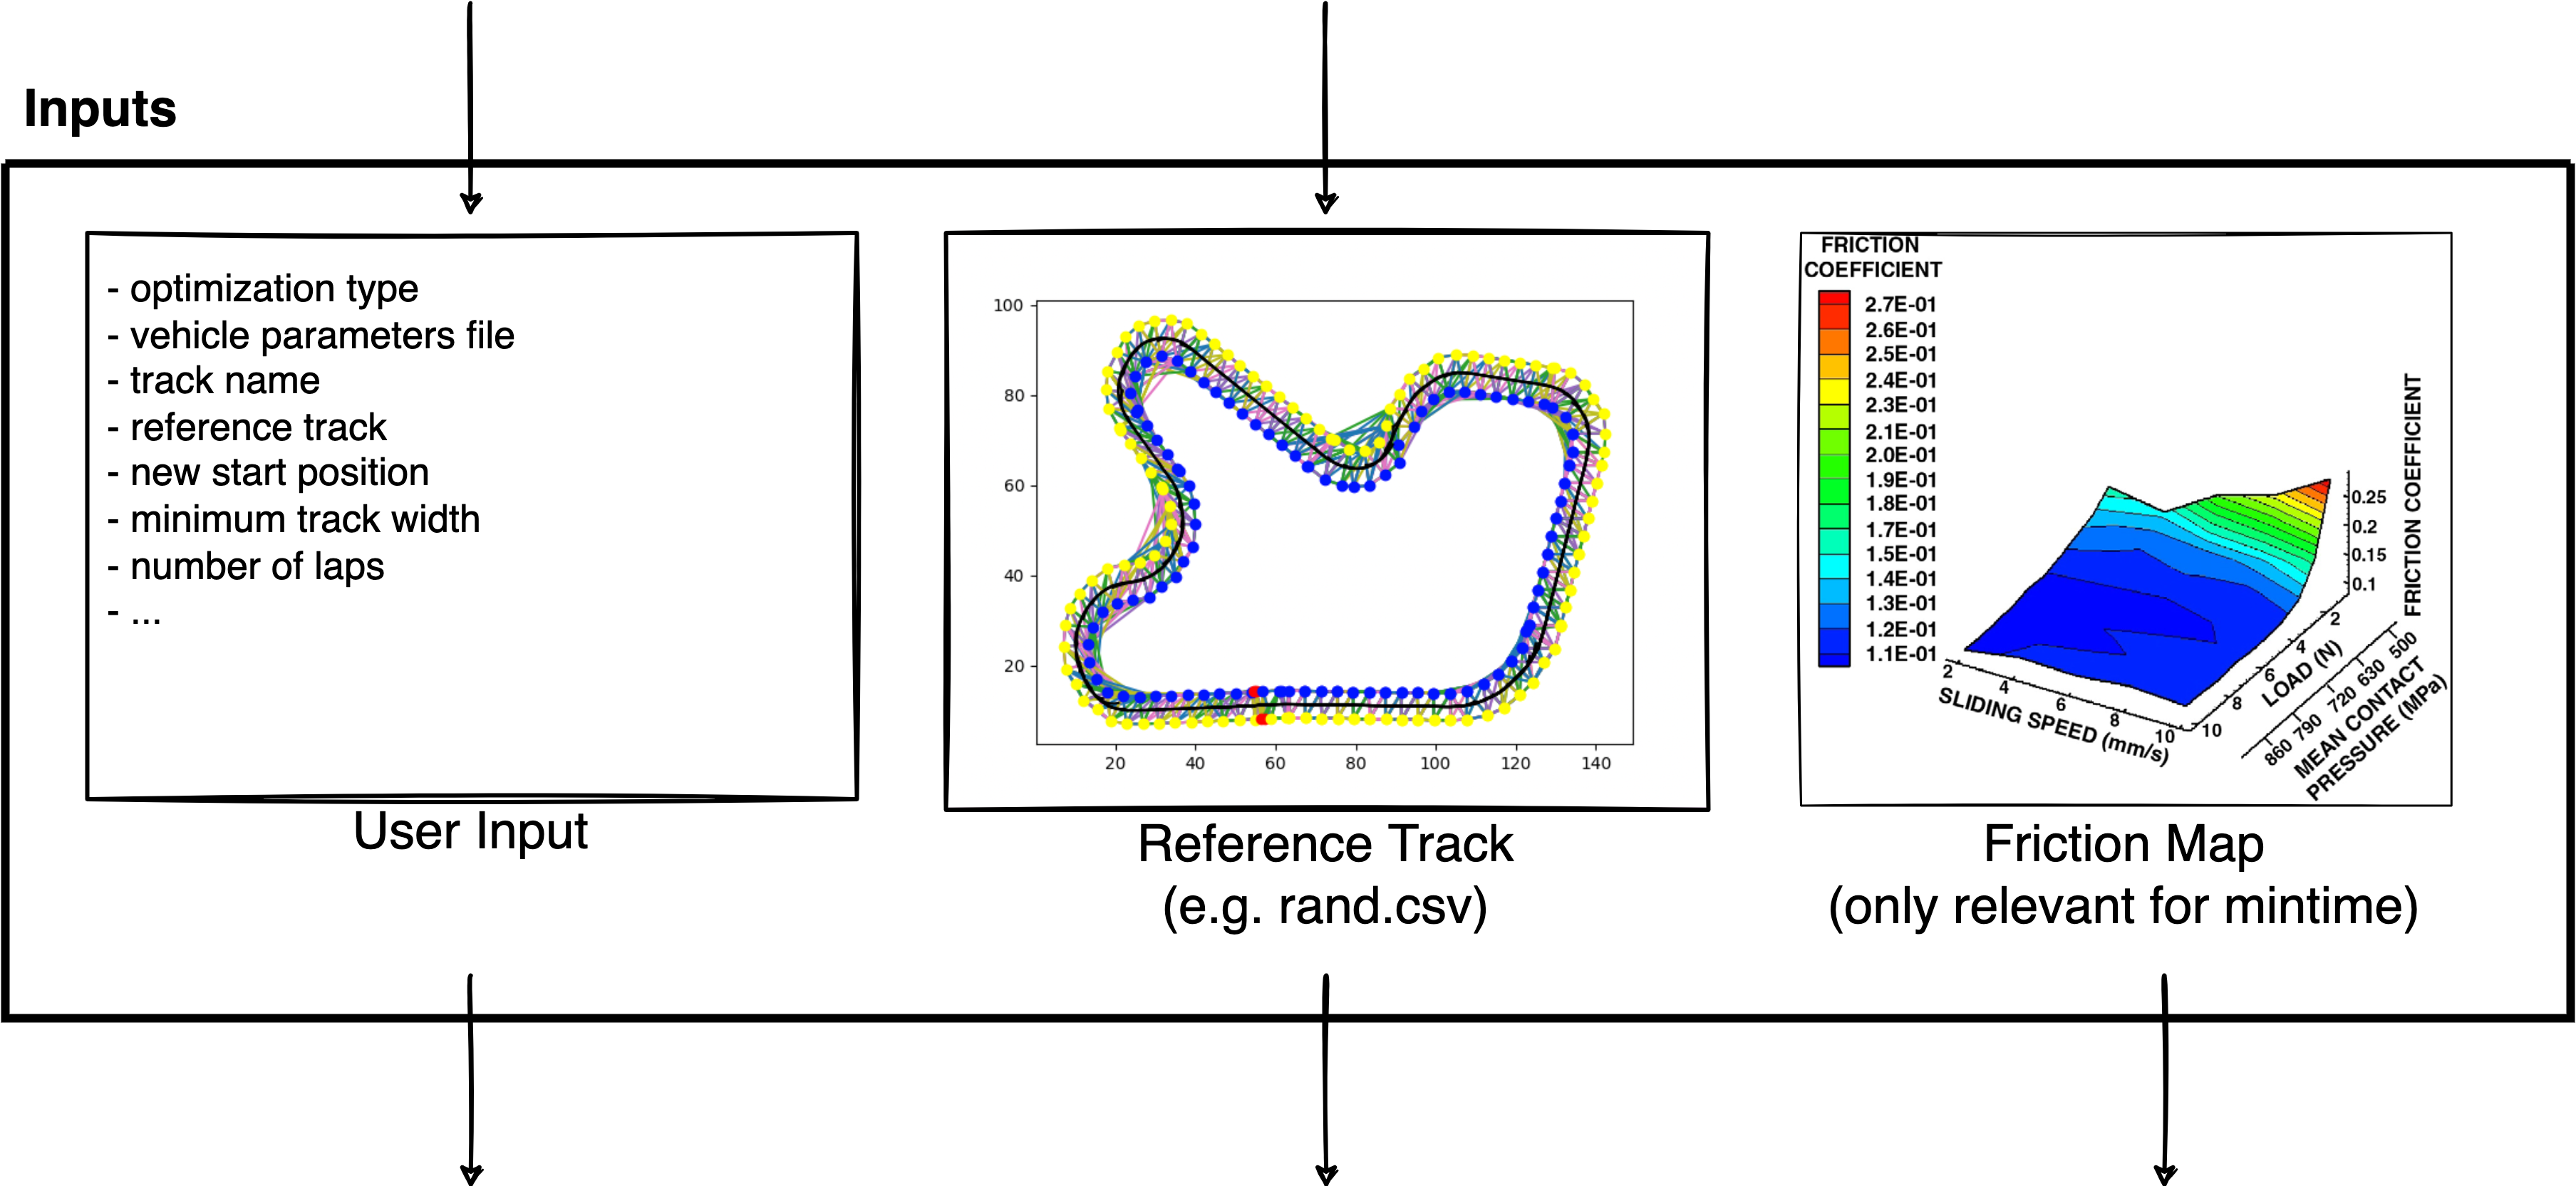
\includegraphics[width=\columnwidth]{Algorithm_Optimization_Module_Inputs.png}
    \caption{The client will receive the user input and reference track. The inputs are the same as seen in figure \ref{fig:Optimization Algorithm Module Overview} but centred horizontally here for better display. The friction map is optional and currently only relevant for Minimum Time solutions.}
    \label{fig:Optimization Algorithm Module Inputs}
\end{figure}

Contained in the ``frictionmap'' package of the project, functions related to the creation and handling of friction maps along the racetrack are provided.
The script contained in ``main\_gen\_frictionmap.py'' can be used to create custom friction maps for any racetrack supplied. The explanation behind the friction map generation is out of scope in this thesis. However, it is explained in detail in ``A Concept for Estimation and Prediction of the Tire-Road Friction Potential for an Autonomous Racecar'' by L. Hermansdorfer, J. Betz and M. Lienkamp. \cite{friction_map_generation}
\begin{figure}[H]
    \centering
    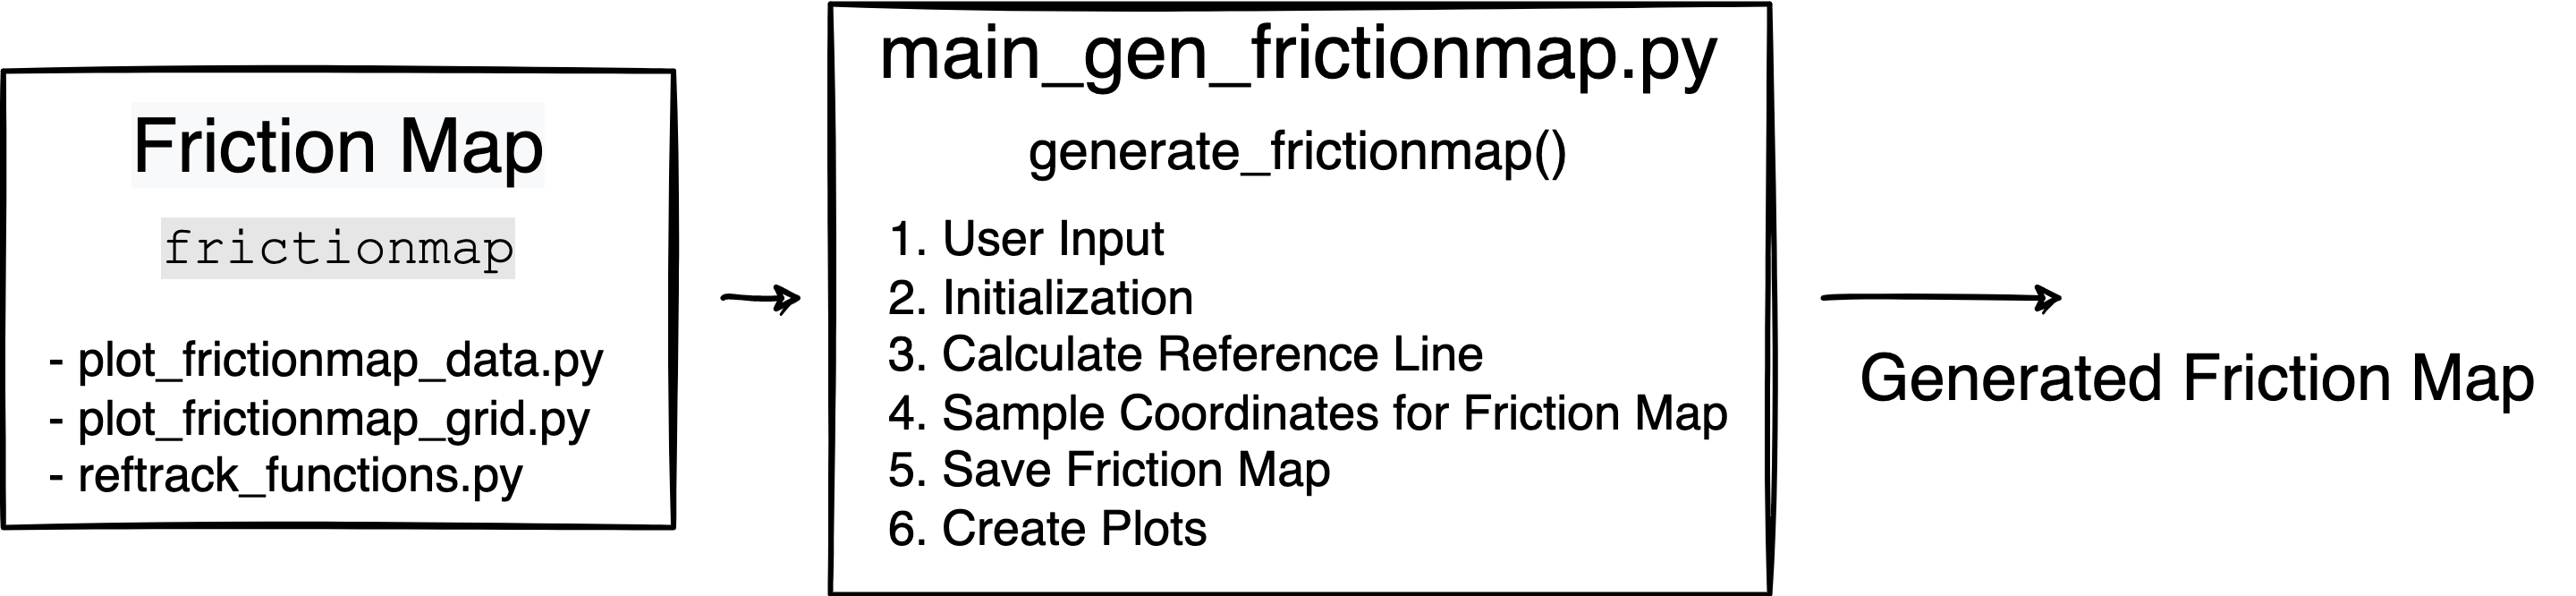
\includegraphics[width=\columnwidth]{Algorithm_Optimization_Module_FrictionMap.png}
    \caption{Overview of the Friction Map package containing functions related to the handling and creation of friction maps as seen in figure \ref{fig:Optimization Algorithm Module Overview}, but centred horizontally here for better display.}
\end{figure}

\textbf{Parameters}

Parameter-wise, the primary method receives everything it needs by the vehicle parameter file called ``racecar.ini''. This file holds general vehicle parameters like the maximum vehicle speed, the vehicle's length, width and mass, its drag coefficient, and its curvature limit. Additionally, the parameter file also holds several calculation options like the step size used for interpolations, smoothing options for spline regression and more.

The vehicle parameter file also sets vehicle dynamics information to be loaded from several files. From a supplementary GGV diagram (``ggv.csv''), also known as the performance envelope, and from a supplementary file called ``ax\_max\_machines.csv'', containing an array with the longitudinal acceleration limits by the electrical motors, as seen in figure \ref{fig:Optimization Algorithm Module Parameters}. If a GG diagram shows the acceleration, a car can achieve at a given speed. Then a GGV diagram would show the maximum acceleration a car can sustain in any horizontal direction when travelling at any speed. The driver's task would then be to take the car to the boundaries of its performance envelope at every moment, while the task of the engineers would be to expand the car's performance envelope by improving its tires, aerodynamics, powertrain and more. \cite{the_performance_envelope_or_ggv_diagram}
\begin{figure}[H]
    \centering
    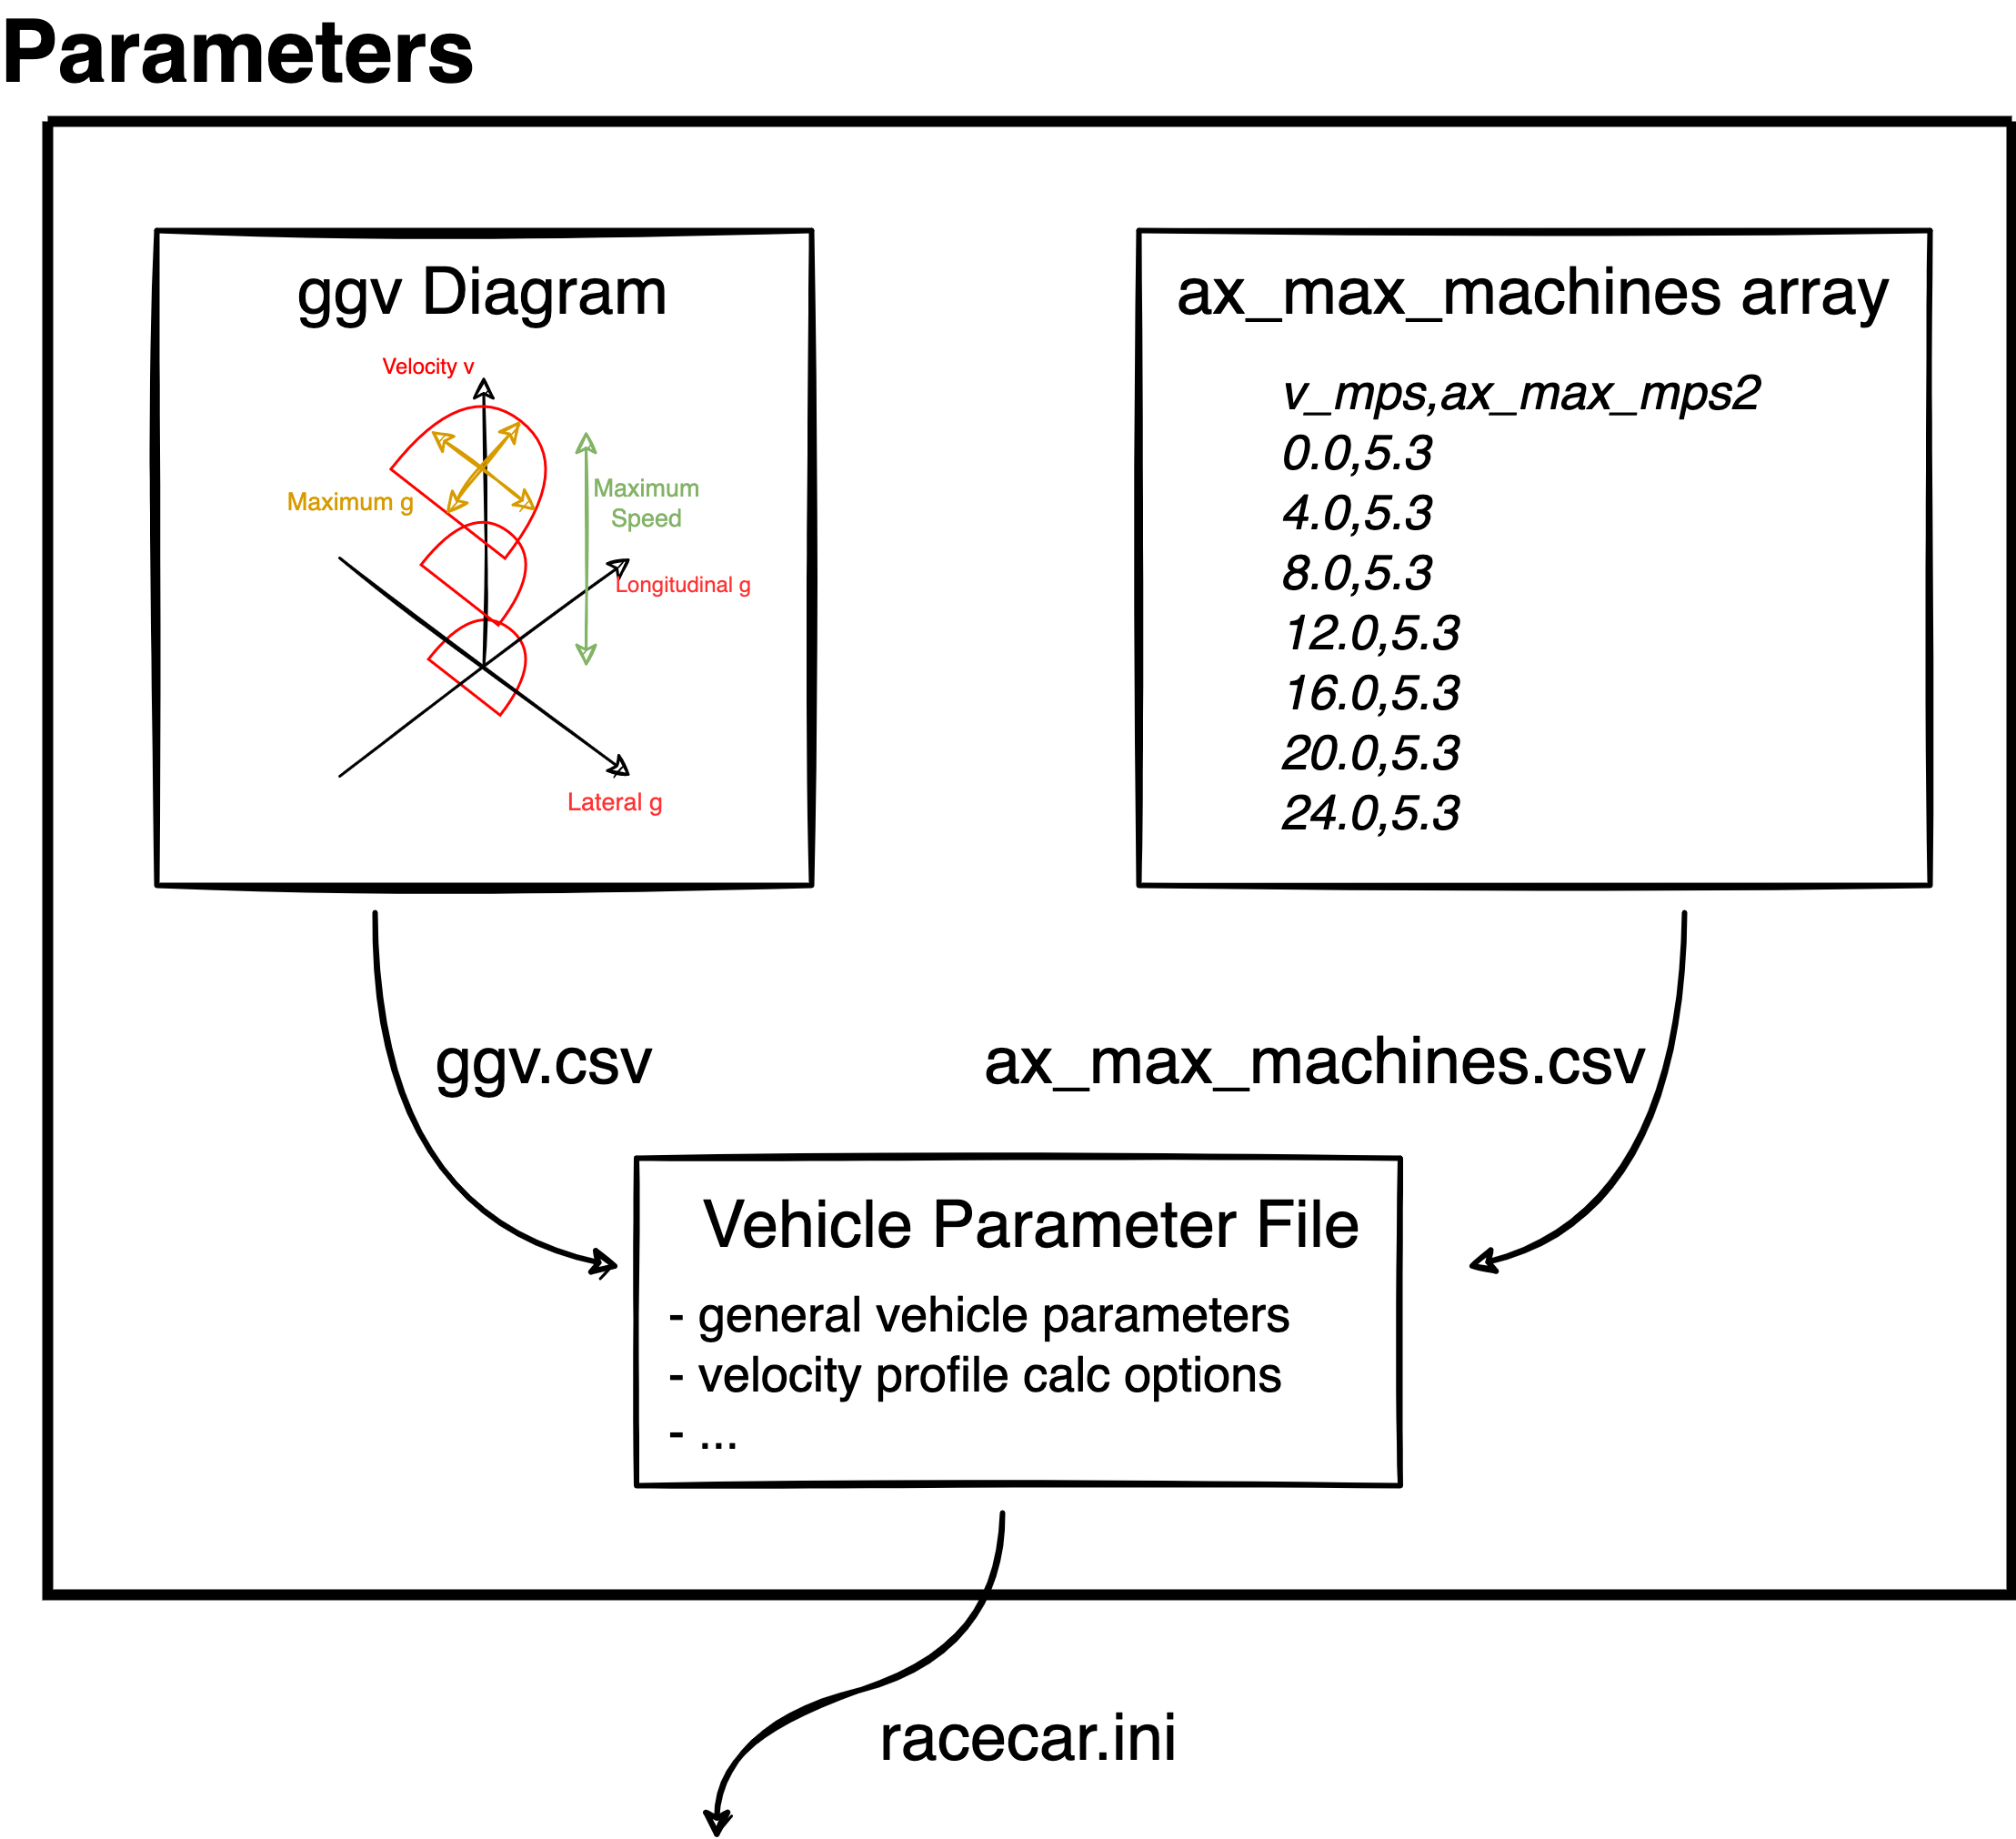
\includegraphics[width=12cm]{Algorithm_Optimization_Module_Parameters.png}
    \caption{Overview of the parameters as seen in figure \ref{fig:Optimization Algorithm Module Overview}. The vehicle parameter file, holding general vehicle parameters and several calculation options, receives additional data from the GGV diagram and the ax machines array.}
    \label{fig:Optimization Algorithm Module Parameters}
\end{figure}

\textbf{1. Import and Initializations}

The primary method will first load, set and check the input provided by the user. After that, all critical paths to the parameter file, output destinations and more will be initialized. Furthermore, the vehicle dependent parameters can be imported from the ``racecar.ini'' file. The additional vehicle dynamics data will be imported by the ``import\_veh\_dyn\_info()'' helper function. The helper function ``import\_track()'' then imports the track itself, with the input provided by the Optimization Input Transformer.

\textbf{2. Prepare Track}

At the next step, the imported track needs to be prepared for optimization by calling the ``prep\_track()'' utility function.

Firstly, it interpolates the reference track by obtaining a smoothed track based on a spline approximation. Secondly, it calculates the splines by solving for curvature continuous cubic splines between the given points.
\begin{figure}[H]
    \centering
    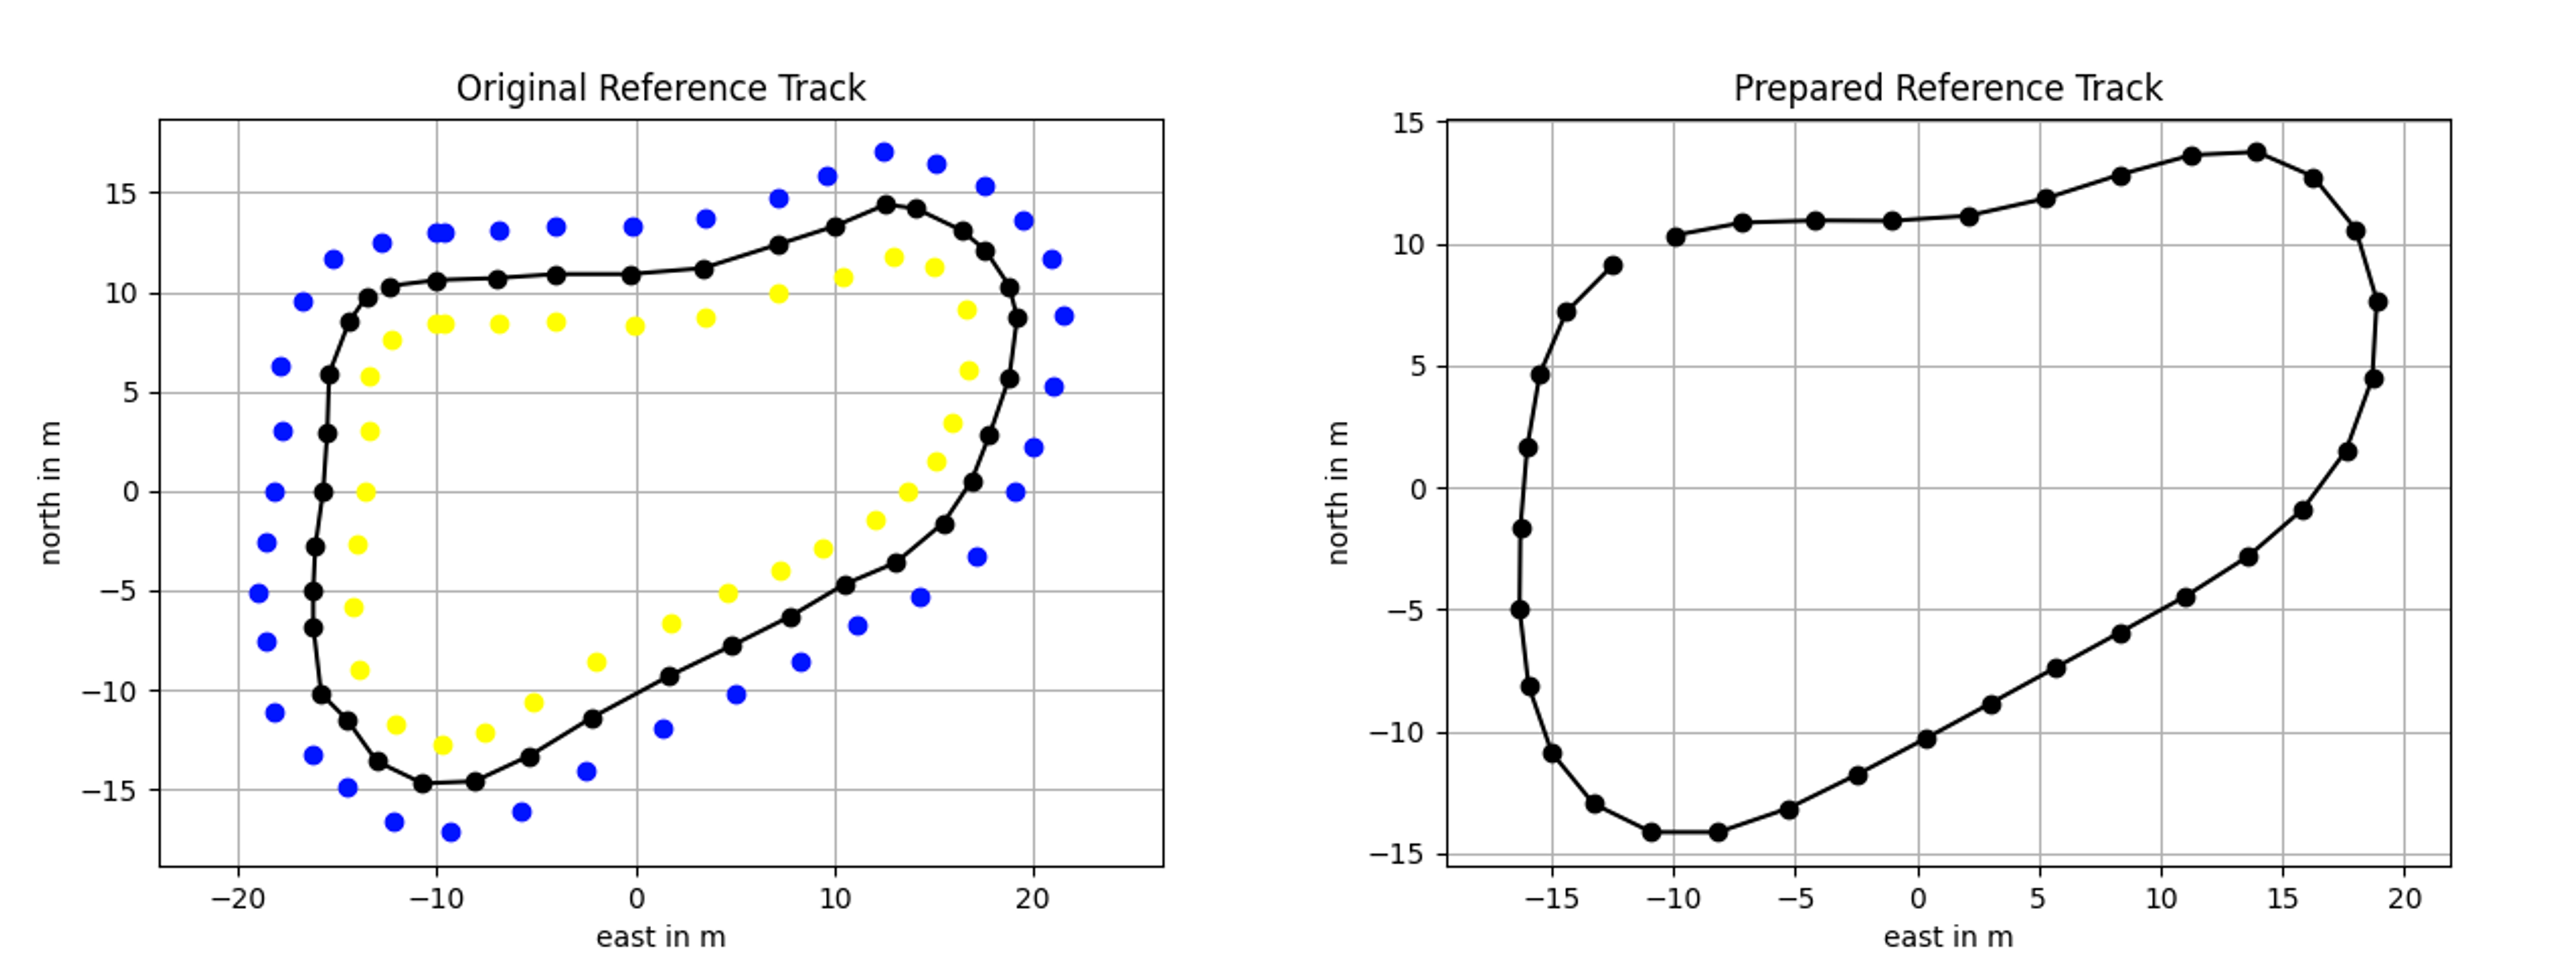
\includegraphics[width=\columnwidth]{Algorithm_Optimization_Prep_Track.png}
    \caption{Side-by-side comparison of the original reference track and the prepared reference track after the spline approximation and calculation for the ``Small Track'' test track.}
    \label{fig:Optimization Algorithm Prepare Track}
\end{figure}
The normal vectors (spline normals) are checked for crossing points to ensure a solution is possible.
\begin{figure}[H]
    \centering
    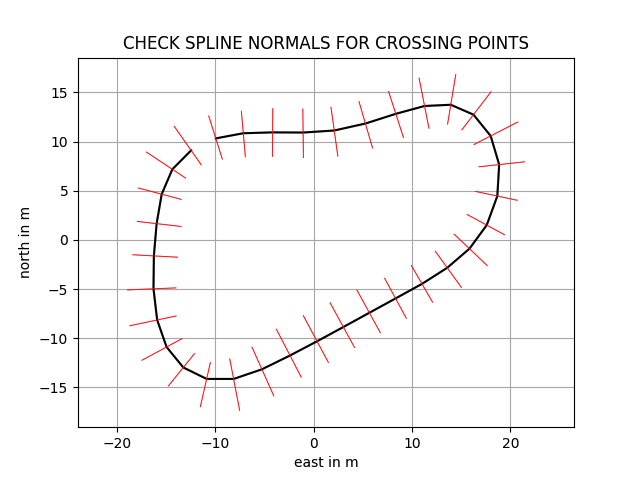
\includegraphics[width=10cm]{Algorithm_Optimization_Check_Splines.png}
    \caption{The spline normals (normal vectors) are checked for crossing points on the ``Small Track'' test track.}
    \label{fig:Optimization Algorithm Check Spline Normals for Crossing Points}
\end{figure}
Finally, if no crossings are detected, the minimum track width set by the user is enforced by inflating tighter sections until the desired track width is reached.
\begin{figure}[H]
    \centering
    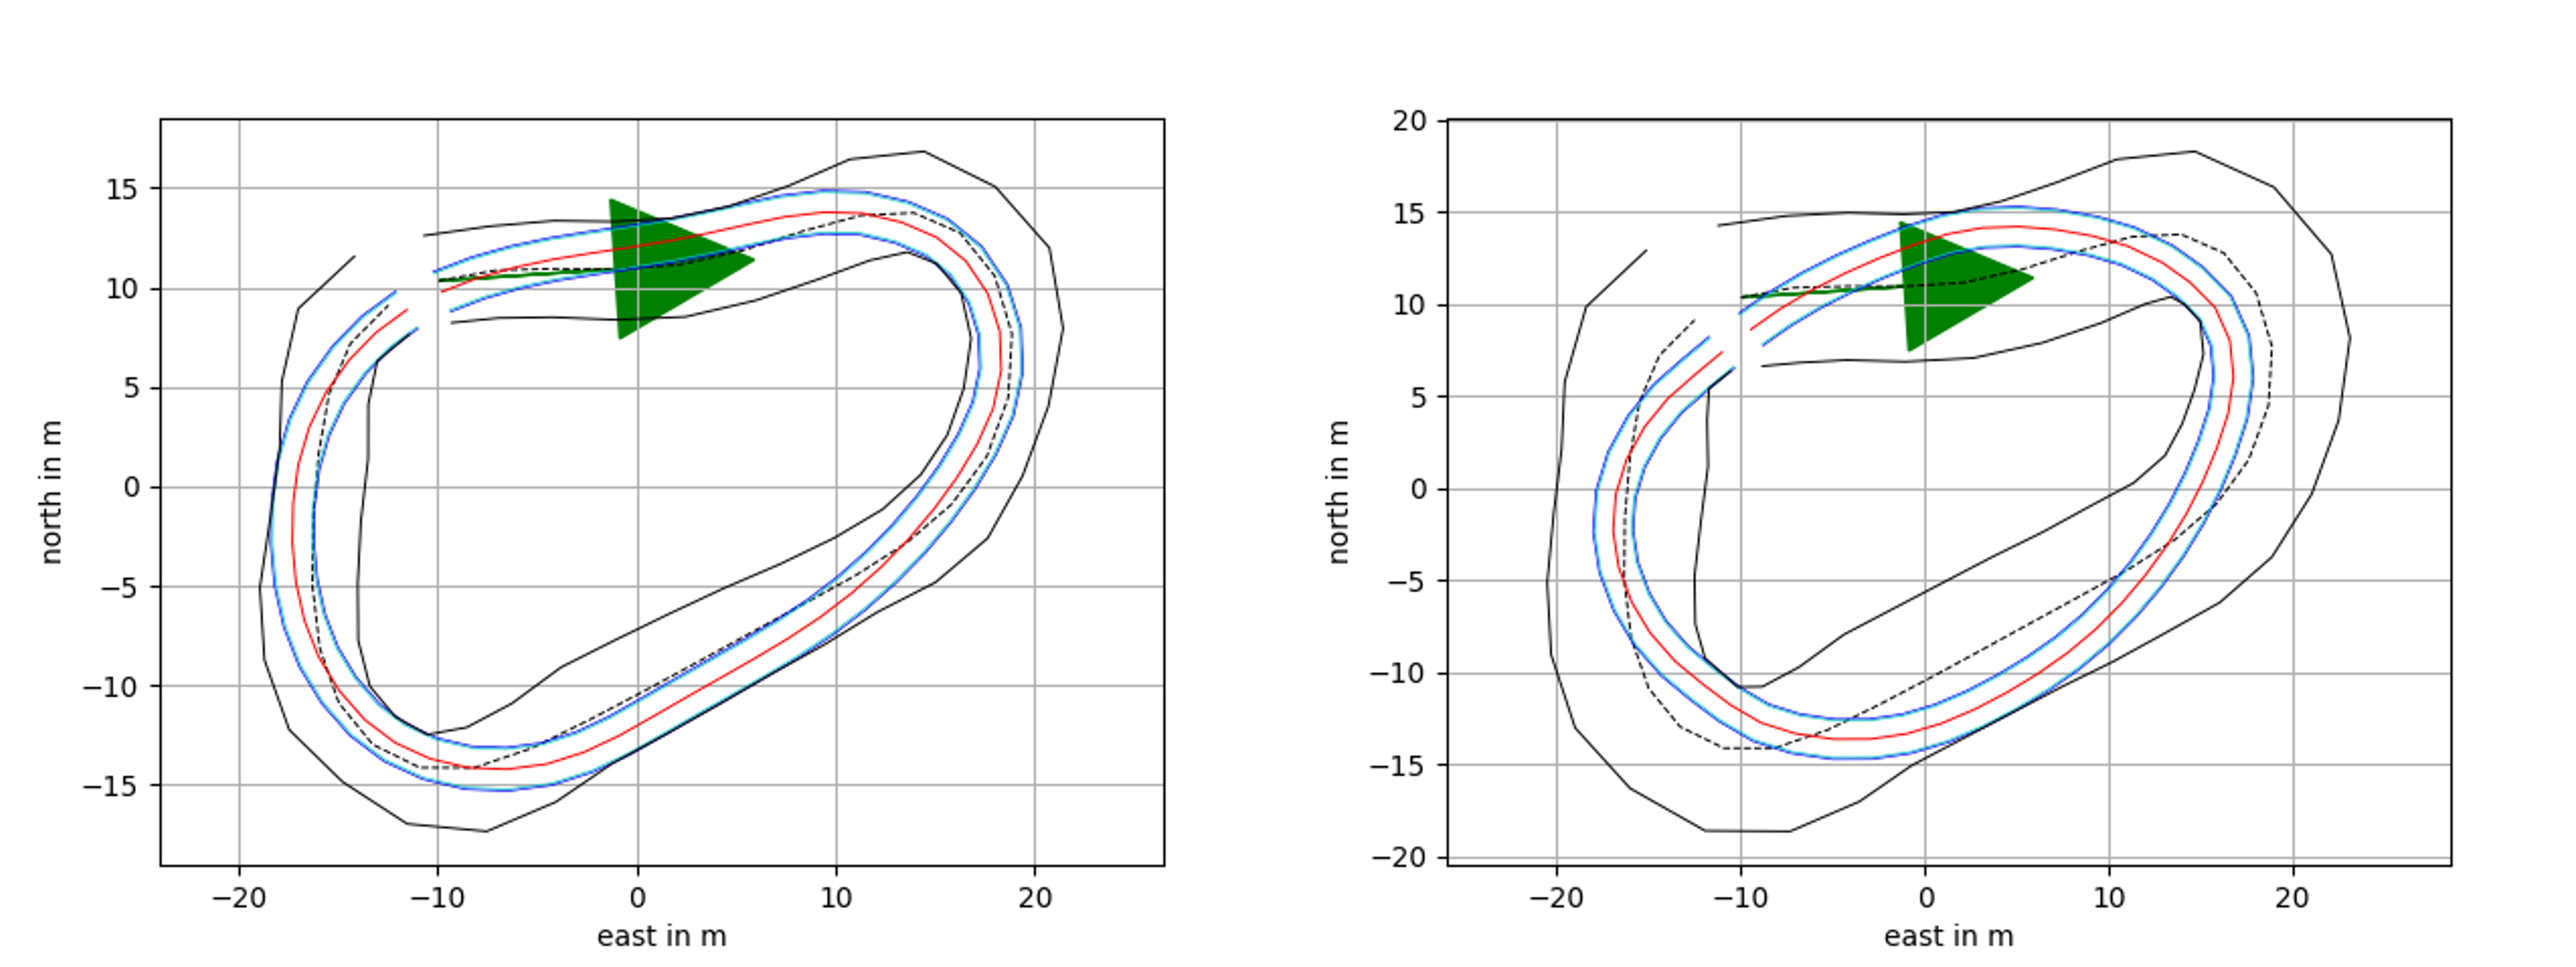
\includegraphics[width=\columnwidth]{Algorithm_Optimization_Enforce_Min_Width.png}
    \caption{Comparison of the ``Small Track'' test track with no minimum track width set (left side) and the same track with an arbitrary high minimum track width set (right side).}
    \label{fig:Optimization Algorithm Enforce minimum width}
\end{figure}

\textbf{3. Call Optimization}

As next, the selected optimization objective gets called: Shortest Path, Minimum Curvature or Minimum Time objective. The solution vector $\alpha$ of the optimization problem containing the lateral shift in m for every point will be returned for each objective.

For \textbf{Shortest Path} optimization, a QP solver is used to minimize the summed length of the path by moving the path points along their normal vectors within the track width. The algorithm is based on the paper ``Race Driver Model'' by F. Braghin, F. Cheli, S. Melzi and E. Sabbioni. \cite{shortest_path}

For \textbf{Minimum Curvature} optimization, a QP solver is used to minimize the summed curvature of the path by moving the path points along their normal vectors within the track width. The algorithm can be used for closed and unclosed tracks. For unclosed tracks, the headings $\psi_s$ and $\psi_e$ are enforced on the first and last point of the reference track. Furthermore, in the case of an unclosed track, the first and last points of the track are not subject to optimization and stay untouched. \cite{minimum_curvature_trajectory_planning}

For \textbf{Minimum Time} optimization, the problem is described as an optimal control problem, converted to a nonlinear program using direct orthogonal Gauss-Legendre collocation and then solved by the interior-point method IPOPT. Reduced computing
times are achieved using a curvilinear abscissa approach for track description, algorithmic differentiation using the software framework CasADi, and the track input data smoothing by approximate spline regression. The vehicle's behaviour is approximated as a double-track model with quasi-steady state tire load simplification and a nonlinear tire model. \cite{minimum_time_trajectory_planning} \cite{powertrain_behaviour}

\begin{figure}[H]
    \centering
    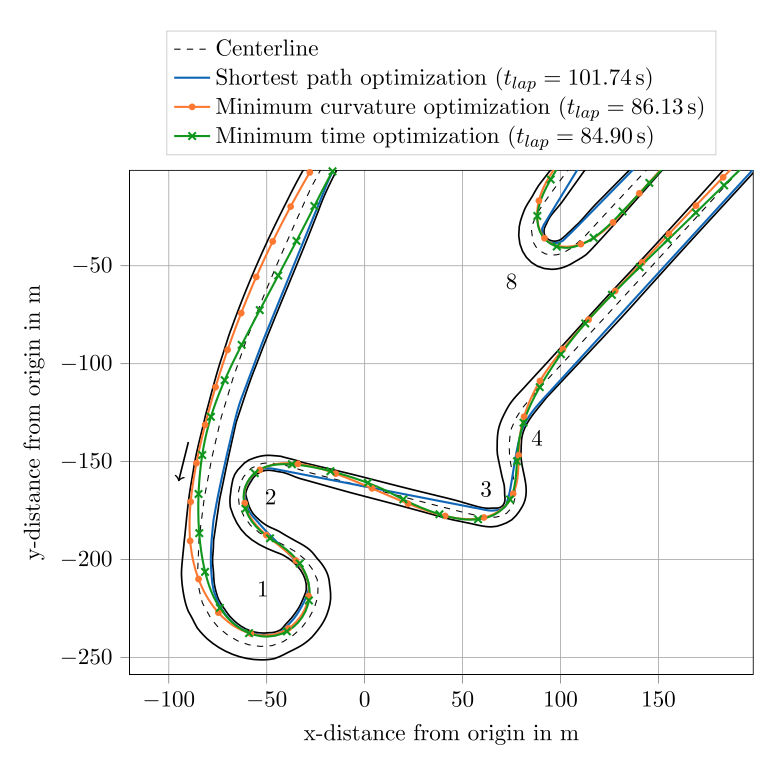
\includegraphics[width=\columnwidth]{Algorithm_Optimization_Comparison_Optimisations.png}
    \caption{Comparison of the paths resulting from the shortest path optimization, minimum curvature optimization and minimum time optimization. \cite{minimum_curvature_trajectory_planning}}
    \label{fig:Optimization Algorithm Comparing Different Optimisations}
\end{figure}

\textbf{4. Create Race Line}

After the optimization call, the race line gets created based on the reference line and the optimization result by interpolating the splines to small distances between the race line points.
\begin{figure}[H]
    \centering
    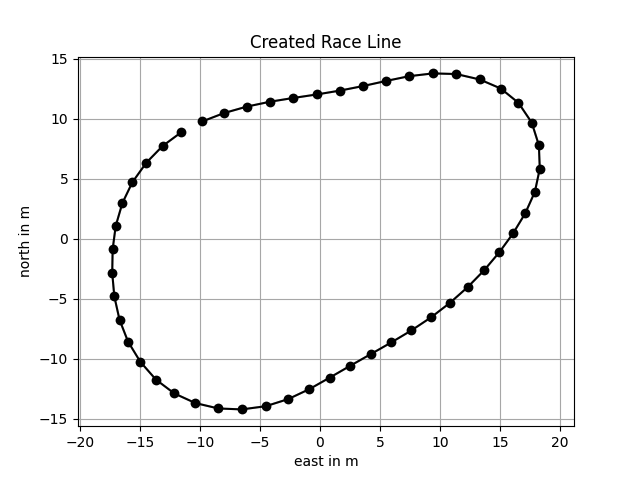
\includegraphics[width=\columnwidth]{Algorithm_Optimization_Create_Raceline.png}
    \caption{The race line was created after interpolating the splines to small distances between the race line points for the ``Small Track'' test track.}
    \label{fig:Optimization Algorithm Created Race Line}
\end{figure}

\textbf{5. Calculate Heading and Curvature}

After that, the analytical calculation of heading $\psi$ and curvature $\kappa$ at every point will be executed.
\begin{figure}[H]
    \centering
    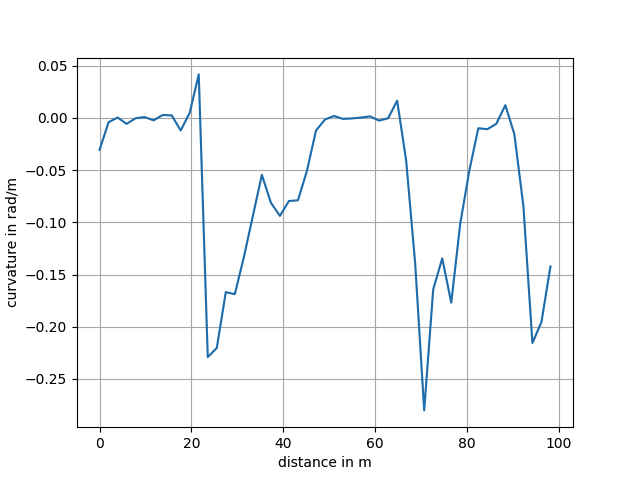
\includegraphics[width=\columnwidth]{Algorithm_Optimization_Curv_Profile.png}
    \caption{The curvature profile of the optimized path for the ``Small Track'' test track.}
    \label{fig:Optimization Algorithm Curvature Profile}
\end{figure}

\textbf{6. Calculate Velocity and Acceleration Profile}

Then the velocity profile will be created, considering the tire and motor limits as good as possible. The longitudinal acceleration profile will then be created for the just created velocity profile. An estimated lap time is calculated within the temporal duration (time) profile for the given trajectory with both profiles.
\begin{figure}[H]
    \centering
    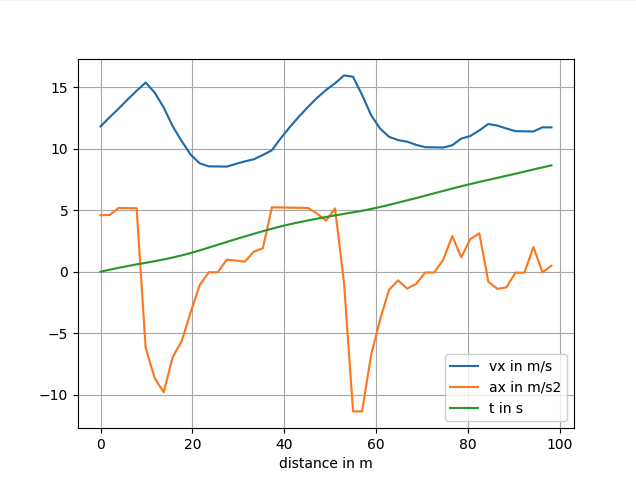
\includegraphics[width=\columnwidth]{Algorithm_Optimization_Vel_Ac_Profile.png}
    \caption{The velocity and acceleration profile for the optimized path for the ``Small Track'' test track.}
    \label{fig:Optimization Algorithm Velocity and Acceleration Profile}
\end{figure}

\textbf{7. Data Post-processing}

Lastly, the data will be arranged into one trajectory, and a closed race trajectory array will be created. The generated trajectory will be checked regarding minimum distance to the boundaries and maximum curvature and accelerations. Moreover, the final trajectory is returned, and plot figures are created if selected.

\section{Integration and Verification} \label{sec:Integration and Verification}

\begin{itemize}
    \item Tests
    \item Integration (inkl. Switch)
    \item Verifikation über Simulationstool (wie ist das setup aufgebaut, welche strecken wurden getestet)
    \item Verifikation und Validierungen (Code Reviews, Fehlerfälle: Cones gehen verloren, Cones andere Seite entdeckt, allg Fehlerannahmen)
    \item Testing mit Maps, Cone Publisher und Planned Trajectory Subscriber (mocks), utils wie track plotter, trackconfig
\end{itemize}

\subsection{Integration} \label{sec:Integration}
The integration of the 'Exploration' part of the program with the 'Optimization' part was accomplished by the ``Start Finish Detector'' described in section \ref{sec:Start Finish Detector} and the ``Optimize Path'' service connecting them both as seen in figure \ref{fig:Path Planning ROS Architecture}. After the Exploration algorithm calculates the path for the first round, the ``Start Finish Detector'' switches to the Optimization algorithm by sending a request over the ``Optimize Path'' service to the Optimization algorithm. The Optimization algorithm then calculates the optimum path for the rest of the laps and returns them to the planner for publishing to the rest of the system.

After implementing the Path Planner and all of its components, the planner had to be integrated with the rest of the autonomous system.
\acrshort{ros} nodes communicate with each other via the ROS graph using topics, services or actions, as described in section \ref{sec:ROS Graph}. As a result, the planner can be integrated into the rest of the autonomous system by just subscribing to the \acrshort{ros} topics for its inputs and creating a publisher for its output, as seen in figure \ref{fig:Path Planning ROS Architecture}.

\subsection{Verification} \label{sec:Verification}
For verification purposes, the mentioned mock nodes in section \ref{sec:Path Planning Component Architecture} are used. The 'Cone Publisher' publishes the corresponding cones of a given track in a fixed order, e.g. first publishing the start cones (big orange cones) and then alternating between a blue cone and a yellow cone. Via \acrshort{ros} parameters, one can select the track to publish, e.g. 'Small Track', 'Skidpad' or 'Acceleration', and the number of laps of a given track to publish in total. On the other hand, the 'Planned Trajectory Subscriber' receives the published trajectories by the Path Planner and logs them to the console. These nodes ensure that all required inputs are generated and dispatched and that the required output is published and acquired.

\subsubsection{Visual Verification with Plots} \label{sec:Visual Verification with Plots}
Plots of the resulting paths and given tracks were created with the ``Matplotlib'' library for Python. The library can plot points, graphs and many other structures on a coordinate system. Verification has been done first and foremost visually with these plots in Python.

\textbf{Exploration Algorithm}

During verification, every algorithm step is plotted on a ``Matplotlib'' figure: Each received cone by the publisher and the resulting triangles during the Delaunay triangulation and the resulting middle points. After implementing the path smoothening with spline interpolation, the resulting smoothed middle lines were plotted instead of the middle points. The test results are found in detail in chapter \ref{ch:Results}. An example of the plots with just the middle points and with the interpolated middle line is found in figure \ref{fig:Verification Visual Plots Exploration}.

\begin{figure}[H]
    \centering
    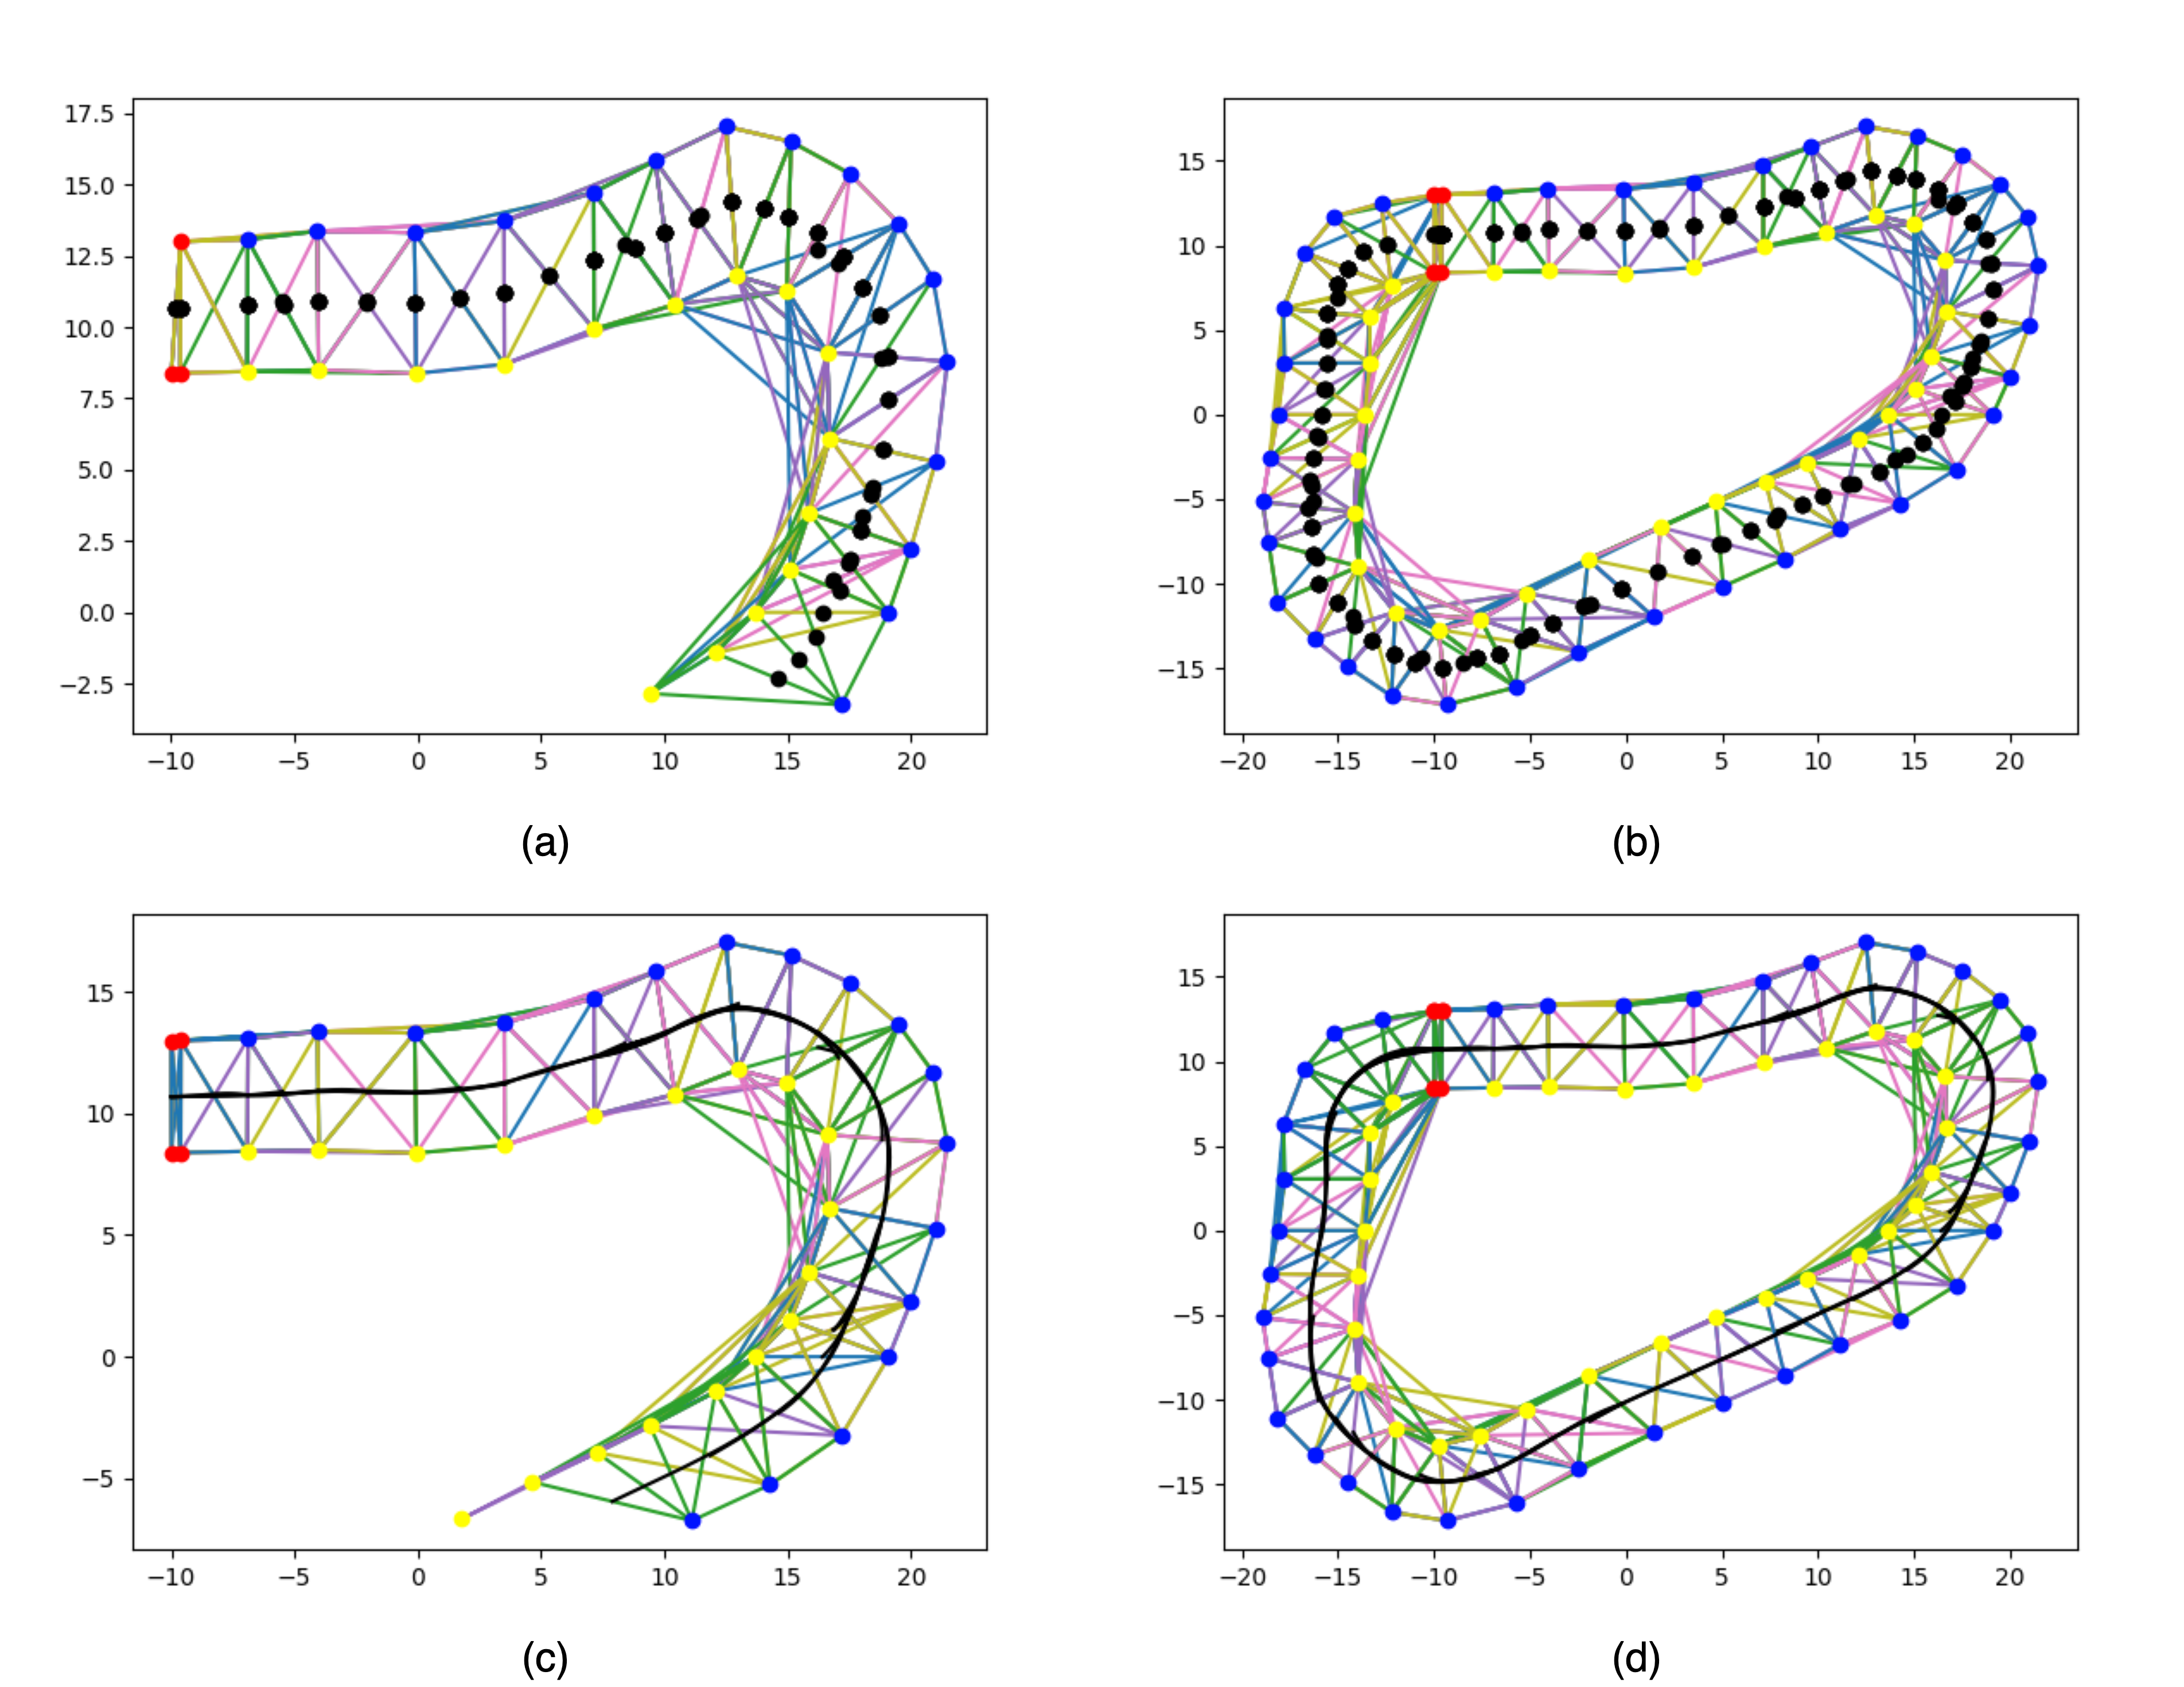
\includegraphics[width=\columnwidth]{Verification_Visual_Plots_Exploration.png}
    \caption{Figures (a) and (b) show a plot of the 'Small Track' with the middle points. The start cones (big orange cones) are red, blue cones are blue, yellow cones are yellow, the middle points are black, and the triangles from triangulation are a variety of colours. Figures (c) and (d) show the same with the interpolated middle line.}
    \label{fig:Verification Visual Plots Exploration}
\end{figure}

\textbf{Optimization Algorithm}

The optimization algorithm was first verified with hard-coded cones given by a track file and a reference line tracked by hand. The 'Optimization Input Transformer', as described in section \ref{sec:Optimization Input Transformer}, converted the inputs to the needed format before letting it optimized by the optimization algorithm. Additionally, the algorithm outputs a velocity and acceleration profile and a curvature profile for the given track. An example of a plot of the optimization algorithm is given in figure \ref{fig:Verification Visual Plots Optimization}.

\begin{figure}[H]
    \centering
    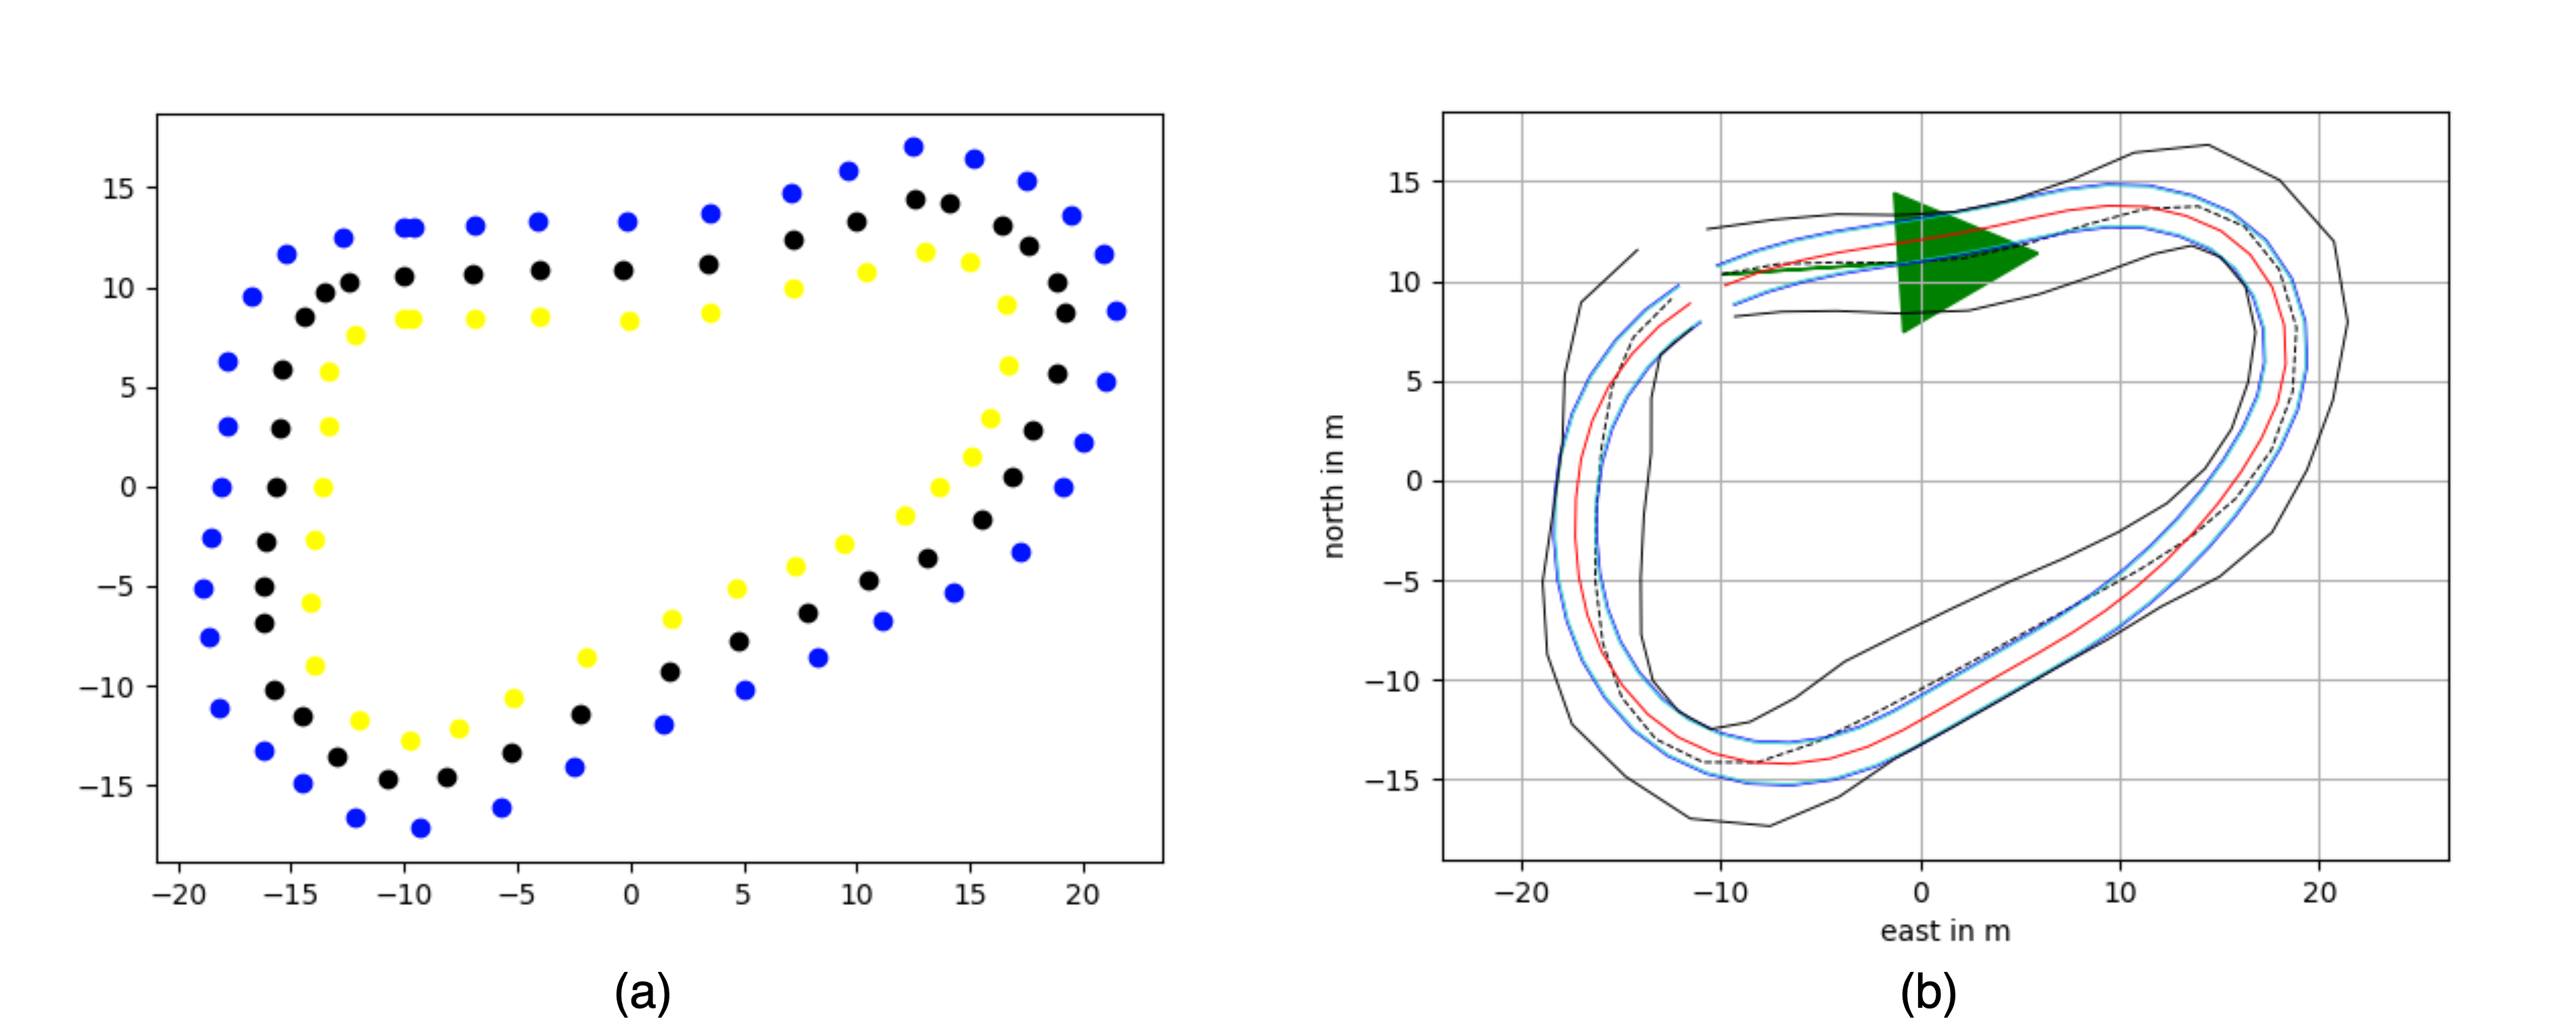
\includegraphics[width=\columnwidth]{Verification_Visual_Plots_Optimization.png}
    \caption{Figure (a) shows the 'Small Track' test track with a predefined reference line by hand. Figure (b) shows the resulting optimized path by the Optimization algorithm.}
    \label{fig:Verification Visual Plots Optimization}
\end{figure}

\subsubsection{Verification with the Simulation Tool} \label{sec:Verification with the Simulation Tool}


